\documentclass[12pt]{article}

\usepackage[margin=1in]{geometry}
\usepackage{graphicx}
\usepackage{booktabs}
\usepackage{array}
\usepackage{amsmath}
\usepackage{float}
\usepackage{hyperref}
\usepackage{xcolor}
\usepackage{listings}
\usepackage{caption}
\usepackage{setspace}
\usepackage{enumitem}
\usepackage[protrusion=true,expansion=true,activate={true,nocompatibility},final,tracking=true,kerning=true,spacing=true,disable={footnote}]{microtype}
\usepackage{fancyhdr}
\usepackage{multirow}

\setstretch{1.25}

\setlength{\parindent}{0pt}
\setlength{\parskip}{0.65em}

\setlist[itemize]{
    leftmargin=1.8em,
    itemsep=0.25em,
    topsep=0.4em
}

\setlist[enumerate]{
    leftmargin=1.8em,
    itemsep=0.25em,
    topsep=0.4em
}

\pagestyle{fancy}
\fancyhf{}
\fancyhead[L]{ENGI-9839 Final Project}
\fancyhead[R]{MD Abdul Hadi Chowdhury}
\fancyfoot[C]{\thepage}

\renewcommand{\headrulewidth}{0.4pt}
\renewcommand{\footrulewidth}{0pt}

\fancypagestyle{plain}{
    \fancyhf{}
    \fancyfoot[C]{\thepage}
    \renewcommand{\headrulewidth}{0pt}
    \renewcommand{\footrulewidth}{0pt}
}
\hypersetup{
    colorlinks=true,
    linkcolor=black,
    citecolor=black,
    urlcolor=blue,
    pdftitle={
        Manual Testing vs. Automated Verification:
        A Comparative Adequacy Study Using Mutation Score
    },
    pdfauthor={MD Abdul Hadi Chowdhury}
}

\lstset{
    basicstyle=\ttfamily\small,
    breaklines=true,
    frame=single,
    numbers=left,
    numberstyle=\tiny,
    showstringspaces=false,
    columns=fullflexible
}

\begin{document}

% =========================================================
% Title Page
% =========================================================

\begin{titlepage}
    \thispagestyle{empty}

    \begin{center}

        \vspace*{1.2cm}

        {\Large
        \textbf{Memorial University of Newfoundland}
        }

        \vspace{0.3cm}

        {\large
        Faculty of Engineering and Applied Science
        }

        \vspace{1.8cm}

        {\Large
        \textbf{ENGI-9839}\\
        Software Verification and Validation
        }

        \vspace{1.6cm}

        \rule{\textwidth}{0.8pt}

        \vspace{0.6cm}

        {\LARGE
        \textbf{Manual Testing vs. Automated Verification}
        }

        \vspace{0.4cm}

        {\Large
        \textbf{A Comparative Adequacy Study Using Mutation Score}
        }

        \vspace{0.6cm}

        \rule{\textwidth}{0.8pt}

        \vspace{1.8cm}

        {\large
        Course Project Report
        }

        \vfill

        \begin{tabular}{rl}
            \textbf{Student Name:} &
            MD Abdul Hadi Chowdhury \\[0.3cm]

            \textbf{Student ID:} &
            202583341 \\[0.3cm]

            \textbf{Course:} &
            ENGI-9839 \\[0.3cm]

            \textbf{Instructor:} &
            Raja Abbas \\[0.3cm]

            \textbf{Submission Date:} &
            July 2026
        \end{tabular}

        \vfill

    \end{center}
\end{titlepage}

% =========================================================
% Front Matter
% =========================================================

\pagenumbering{roman}
\pagestyle{plain}

\section*{Abstract}
\addcontentsline{toc}{section}{Abstract}

This study compares the adequacy of two software testing approaches applied to
the financial transaction subsystem of an open-source Django banking
application. The first approach used manually designed pytest test cases based
on equivalence partitioning and boundary value analysis. The second approach
used property-based testing with Hypothesis to generate inputs from financial
requirements and invariants.

Both test suites were evaluated against the same pinned version of the subject
system and the same mutation-testing scope. Structural coverage was measured
using \texttt{pytest-cov}, while fault-detection adequacy was assessed using
\texttt{mutmut}. The manual suite contained 29 test functions and achieved
84\% coverage. The property-based suite contained 16 property test functions
and achieved 77\% coverage.

The \texttt{mutmut} tool generated 96 mutants in each experimental run. Twenty-six mutants belonged to an out-of-scope transaction date-range
form and were excluded consistently from the controlled comparison. This left
70 relevant mutants. The manual suite killed 53 relevant mutants, resulting in
a controlled mutation score of 75.71\%. The property-based suite killed 42
relevant mutants, resulting in a controlled score of 60.00\%.

When only mutants reached by each suite were considered, the scores were much
closer: 75.71\% for the manual suite and 73.68\% for the property-based suite.
This indicates that the main difference was behavioural reach rather than a
large difference in fault-detection strength within executed code. Survivor
analysis also identified shared weaknesses in interest arithmetic, currency
rounding, and interest-period verification. The findings support using manual
EP/BVA testing and property-based testing as complementary techniques.
\newpage

\tableofcontents

\newpage

\listoftables
\addcontentsline{toc}{section}{List of Tables}

\newpage

\listoffigures
\addcontentsline{toc}{section}{List of Figures}

\newpage

% =========================================================
% Main Report
% =========================================================

\pagenumbering{arabic}
\pagestyle{fancy}

\section{Introduction}

Software testing is a central activity in software verification and
validation because it provides evidence that an implementation behaves
according to its requirements. In practice, test suites are often created
manually using selected input-output examples. Systematic black-box techniques
such as equivalence partitioning and boundary value analysis help testers
choose representative cases from valid, invalid, and boundary regions of the
input domain.

Property-based testing follows a different approach. Instead of defining only
individual examples, the tester expresses general properties that must hold
for many automatically generated inputs. In Python, the Hypothesis framework
supports this style of testing through reusable data strategies, generated
examples, shrinking, and repeated execution of behavioural properties.

Although both approaches can reveal faults, comparing them using only the
number of test functions or code coverage can be misleading. A test suite may
execute a line of code without checking its result strongly enough to detect
an error. Therefore, structural coverage alone does not fully measure
fault-detection adequacy.

Mutation testing provides a stronger evaluation mechanism. It introduces small
syntactic changes into the production code, such as replacing arithmetic
operators, altering constants, or removing function arguments. A mutant is
considered killed when at least one test fails against the modified program.
If all tests continue to pass, the mutant survives. Mutation score therefore
evaluates both execution reach and assertion strength.

In this report, the term \emph{manual suite} refers to manual test-case design,
not manual test execution. Both suites were executed automatically using
\texttt{pytest}. The comparison concerns manually selected EP/BVA examples
versus automatically generated Hypothesis inputs and properties.

This project compares a manually designed EP/BVA test suite with a Hypothesis
property-based test suite for the financial transaction subsystem of an
open-source Django banking application. The selected subsystem includes
deposit validation, withdrawal validation, account balance changes,
transaction-record creation, interest calculation, and selected account-model
behaviour.

The primary research question is:

\begin{quote}
For the selected financial transaction subsystem, how does the mutation
adequacy of a manually designed equivalence-partitioning and boundary-value
test suite compare with that of a Hypothesis property-based test suite?
\end{quote}

The project also addresses the following secondary questions:

\begin{enumerate}
    \item Which suite achieves higher structural coverage?
    \item Which suite reaches a broader range of financial behaviours?
    \item Which categories of mutants survive both test suites?
    \item What relationship is observed between structural coverage and
          mutation adequacy?
\end{enumerate}

The experiment was controlled by using the same subject-system revision,
Python environment, source files, mutation tool, mutation configuration, and
target modules. Only the selected test suite changed between the two mutation
runs.

The main finding is that the manually designed suite achieved the higher
controlled mutation score, primarily because it exercised a broader range of
account and transaction behaviour. However, the two suites achieved similar
scores when only reached mutants were considered. This suggests that the
property-based suite was nearly as effective within the behaviours it tested,
but its property catalogue covered a narrower part of the selected subsystem.

The remainder of this report presents the relevant testing background,
describes the subject system and experimental design, explains both test
suites, reports the coverage and mutation results, analyzes surviving mutants,
and discusses the findings, threats to validity, recommendations, and
conclusion.

% =========================================================
% Background and Related Work
% =========================================================

\section{Background and Related Work}

\subsection{Equivalence Partitioning}

Equivalence partitioning is a specification-based testing technique that
divides an input domain into classes whose members are expected to produce
similar behaviour. Instead of testing every possible value, the tester selects
representative values from valid and invalid partitions.

For the selected banking subsystem, relevant partitions include valid and
invalid deposit amounts, valid and invalid withdrawal amounts, withdrawal
amounts below or above configured limits, and withdrawals that are within or
greater than the available balance.

The main benefit of equivalence partitioning is that it reduces a potentially
large input domain to a manageable set of meaningful test cases. Its
effectiveness depends on whether the tester identifies all important
partitions and selects appropriate representatives.

\subsection{Boundary Value Analysis}

Boundary value analysis focuses on values at, immediately below, and
immediately above important thresholds. Many software defects occur near
boundaries because of incorrect relational operators, off-by-one errors, or
incomplete handling of limiting cases.

Financial applications contain several important boundaries. In this project,
the most relevant examples were:

\begin{itemize}
    \item the minimum accepted deposit amount;
    \item the minimum withdrawal amount;
    \item the maximum withdrawal amount; and
    \item the current account balance.
\end{itemize}

The manually designed suite therefore included cases below, at, and above
these thresholds wherever applicable.

\subsection{Property-Based Testing}

Property-based testing expresses expected behaviour as general rules rather
than only as fixed input-output examples. A property is evaluated repeatedly
using automatically generated inputs. QuickCheck popularized this approach by
combining generators, executable properties, and shrinking of failing
examples \cite{hughes2010quickcheck}.

The Python framework Hypothesis follows this model. Test data is generated
from reusable strategies, and each property test may execute many examples.
When a failure is found, Hypothesis attempts to reduce it to a simpler
counterexample.

Property-based testing is especially useful when a requirement can be
expressed as an invariant. Examples from the selected banking subsystem
include:

\begin{itemize}
    \item an accepted deposit must not reduce the account balance;
    \item an accepted withdrawal must reduce the balance by exactly the
          withdrawal amount;
    \item an invalid transaction must not modify financial state; and
    \item interest should remain non-negative for valid positive inputs.
\end{itemize}

However, automatic input generation cannot compensate for a missing property.
Behaviour that is not represented in the property catalogue will not be tested,
regardless of how many values are generated.

\subsection{Structural Coverage}

Structural coverage measures which parts of the implementation are executed by
a test suite. Common metrics include statement coverage and branch coverage.

Coverage is useful for identifying unexecuted code, but it does not directly
measure whether the tests can detect incorrect behaviour. A statement may be
executed without any assertion checking its result. Therefore, a high coverage
percentage does not necessarily imply a strong test oracle.

In this project, coverage was used as a secondary adequacy measure. The primary
comparison was based on mutation testing.

\subsection{Mutation Testing}

Mutation testing introduces small syntactic modifications into production
code. Each modified version is called a mutant. Typical mutation operators
replace arithmetic operators, alter constants, remove arguments, or change
return expressions.

A mutant is classified as killed when at least one test fails against it. A
mutant survives when all tests still pass. Surviving mutants may indicate weak
assertions, incomplete input selection, underspecified behaviour, or semantic
equivalence with the original program.

Mutation testing has been widely studied as a fault-based test adequacy
criterion \cite{jia2011mutation}. It evaluates both whether code is reached and
whether the test oracle is capable of detecting a behavioural change.

A conventional mutation score may exclude confirmed equivalent mutants:

\begin{equation}
MS =
\frac{K}{M-E}
\times 100,
\end{equation}

where:

\begin{itemize}
    \item \(K\) is the number of killed mutants;
    \item \(M\) is the total number of generated mutants; and
    \item \(E\) is the number of confirmed equivalent mutants.
\end{itemize}

Equivalent mutants are syntactically different from the original program but
produce the same observable behaviour for all relevant inputs. Because they
cannot be distinguished from the original program through observable test
outcomes, confirmed equivalent mutants may be excluded from a conventional
mutation score.

In this study, the two mutants classified as equivalent or likely equivalent
were not removed from the reported scores because their equivalence was not
formally proven. Instead, the study reported a separate controlled
relevant-population score that consistently excluded 26 mutants belonging to
the declared out-of-scope transaction date-range functionality.

Mutation score should not be interpreted as a perfect substitute for real
fault detection. Prior empirical research has shown that test-suite size and
other confounding factors may influence observed relationships between
mutation score and real defects \cite{papadakis2018mutation}.

\subsection{Related Empirical Work}

Recent empirical research has examined property-based testing in Python
projects and evaluated its effectiveness using mutation analysis
\cite{ravi2025property}. Such work suggests that the effectiveness of
property-based testing depends strongly on the quality and scope of the
properties being tested.

This project extends that line of inquiry through a controlled case study of a
financial Django subsystem. The study compares two independently designed test artifacts against the same
source revision, mutation targets, and mutation configuration.

% =========================================================
% Subject System and Experimental Scope
% =========================================================

\section{Subject System and Experimental Scope}

\subsection{Selected Subject System}

The subject system selected for this study was the open-source
\texttt{saadmk11/banking-system} project \cite{bankingsystem}. The application is implemented in
Python using the Django web framework and provides banking-related
functionality such as account management, deposits, withdrawals, transaction
records, interest calculation, and transaction reporting.

The project was selected because it contains realistic financial rules and
state-changing operations suitable for software verification and testing.
Financial software is especially appropriate for this study because small
arithmetic, validation, or boundary errors may lead to incorrect balances or
invalid transactions.

The upstream repository was imported into the project under:

\begin{verbatim}
subject_system/banking_system/
\end{verbatim}

To ensure reproducibility, the evaluated source was pinned to the following
upstream commit:

\begin{verbatim}
9c3ee3eea75030280405506c62d968d646981c05
\end{verbatim}

The source repository and pinned revision were documented in
\texttt{subject\_system/UPSTREAM.md}.

\subsection{Original Testing Condition}

The original project contained test modules under the account and transaction
applications. However, these modules did not contain executable test cases.
Running the original Django test command collected zero tests.

Therefore, the two test suites evaluated in this study were developed
specifically for the experiment:

\begin{enumerate}
    \item a manually designed pytest suite based on equivalence partitioning
          and boundary value analysis; and
    \item a Hypothesis property-based test suite derived from financial
          requirements and invariants.
\end{enumerate}

No existing executable tests were reused in either suite.

\subsection{Selected Financial Subsystem}

The full banking application contains functionality beyond the needs of this
study. The experiment therefore focused on a limited financial transaction
subsystem.

The selected behaviour included:

\begin{itemize}
    \item deposit amount validation;
    \item minimum withdrawal validation;
    \item maximum withdrawal validation;
    \item rejection of withdrawals exceeding the available balance;
    \item account balance increases after accepted deposits;
    \item account balance decreases after accepted withdrawals;
    \item preservation of account state after rejected operations;
    \item creation of transaction records;
    \item association of transaction records with the correct account;
    \item storage of the balance after a transaction;
    \item interest calculation;
    \item interest-calculation scheduling; and
    \item selected account-model helper behaviour.
\end{itemize}

The principal source modules examined were:

\begin{table}[H]
\centering
\caption{Source modules included in the verification study}
\label{tab:selected-modules}

\begin{tabular}{|p{5.2cm}|p{8.5cm}|}
\hline
\textbf{Module} & \textbf{Relevant responsibility} \\
\hline

\texttt{accounts/models.py} &
Bank-account types, interest calculation, account balances, and
interest-calculation month scheduling. \\
\hline

\texttt{transactions/forms.py} &
Deposit and withdrawal validation, transaction-form initialization, and
transaction-record preparation. \\
\hline

\texttt{transactions/models.py} &
Transaction data, transaction type, amount, account association, and balance
after transaction. \\
\hline

\texttt{transactions/views.py} &
Deposit and withdrawal processing, balance updates, and transaction
completion. \\
\hline

\end{tabular}
\end{table}

\subsection{Excluded Functionality}

The following functionality was excluded from the experimental scope:

\begin{itemize}
    \item user authentication and authorization;
    \item account registration;
    \item administrative interfaces;
    \item HTML templates and visual presentation;
    \item Celery background tasks;
    \item Redis integration;
    \item email notification behaviour;
    \item transaction report rendering;
    \item transaction date-range filtering; and
    \item deployment and production infrastructure.
\end{itemize}

These exclusions kept the experiment focused on financial correctness rather
than user-interface, infrastructure, or reporting concerns.

\subsection{Financial Rules Observed in the Implementation}

The selected implementation enforces several important financial rules.

A deposit must satisfy the configured minimum-deposit amount. Deposits below
this threshold are rejected. An accepted deposit increases the account balance
by the deposited amount.

A withdrawal must satisfy three conditions:

\begin{enumerate}
    \item it must not be below the configured minimum withdrawal;
    \item it must not exceed the configured maximum withdrawal; and
    \item it must not exceed the current account balance.
\end{enumerate}

An accepted withdrawal reduces the account balance by the requested amount.
A rejected withdrawal must not modify the balance or create an accepted
transaction record.

The implementation also calculates interest using the principal balance,
configured annual interest rate, and number of interest calculations per year.
The result is rounded to two decimal places.

\subsection{Absence of Inter-Account Transfers}

The selected system does not implement a direct transfer operation between two
accounts. Therefore, a traditional inter-account balance-conservation
property could not be tested.

Instead, the study evaluated related financial-state invariants:

\begin{itemize}
    \item accepted deposits increase the balance by exactly the deposited
          amount;
    \item accepted withdrawals decrease the balance by exactly the withdrawn
          amount; and
    \item rejected financial operations preserve the original balance.
\end{itemize}

This adaptation maintained the financial-verification objective without
inventing functionality that was not present in the subject system.

\subsection{Repository Artifact}

The complete project artifact is maintained at:

\begin{center}
\url{https://github.com/hadiChowdhury/Svv-banking-verification-study}
\end{center}

The repository contains the imported subject source, test suites, requirement
documents, invariant catalogue, coverage reports, mutation results,
surviving-mutant details, and scripts required to reproduce the experiment.

% =========================================================
% Requirements, Invariants, and Test Oracles
% =========================================================

\section{Requirements, Invariants, and Test Oracles}

\subsection{Requirements Extraction}

The selected subject system did not provide a complete formal requirements
document for financial transaction behaviour. Therefore, the experiment
first reconstructed the relevant behavioural requirements from the source
code, model configuration, form validation logic, view processing, and
observable transaction outcomes.

The resulting specification was documented in:

\begin{verbatim}
docs/requirements_specification.md
\end{verbatim}

A total of 22 requirements were identified and grouped into the following
categories:

\begin{table}[H]
\centering
\caption{Requirement categories used in the study}
\label{tab:requirement-categories}

\begin{tabular}{|l|c|c|}
\hline
\textbf{Category} & \textbf{Identifier Range} & \textbf{Count} \\
\hline
Deposit requirements & D1--D5 & 5 \\
\hline
Withdrawal requirements & W1--W8 & 8 \\
\hline
Transaction requirements & T1--T4 & 4 \\
\hline
Interest and account requirements & I1--I5 & 5 \\
\hline
\textbf{Total} & & \textbf{22} \\
\hline
\end{tabular}

\end{table}

The requirements were written in terms of externally observable behaviour
wherever possible. This reduced dependence on implementation-specific details
and supported both manual and property-based test design.

\subsection{Deposit Requirements}

The deposit requirements were summarized as follows:

\begin{enumerate}[label=\textbf{D\arabic*:}]
    \item A deposit below the configured minimum must be rejected.
    \item A deposit equal to the configured minimum must be accepted.
    \item A deposit greater than the configured minimum must be accepted.
    \item An accepted deposit must increase the account balance by exactly the
          deposited amount.
    \item A rejected deposit must not modify the account balance or create an
          accepted transaction record.
\end{enumerate}

These requirements support both fixed boundary tests and generalized
properties over generated deposit amounts.

\subsection{Withdrawal Requirements}

The withdrawal requirements were summarized as follows:

\begin{enumerate}[label=\textbf{W\arabic*:}]
    \item A withdrawal below the configured minimum must be rejected.
    \item A withdrawal equal to the configured minimum must be accepted when
          all other conditions are satisfied.
    \item A withdrawal below or equal to the configured maximum may be
          accepted when sufficient funds are available.
    \item A withdrawal greater than the configured maximum must be rejected.
    \item A withdrawal greater than the current balance must be rejected.
    \item A withdrawal equal to the current balance may be accepted when it
          satisfies the configured limits.
    \item An accepted withdrawal must reduce the balance by exactly the
          withdrawal amount.
    \item A rejected withdrawal must preserve the original balance and must
          not produce an accepted transaction.
\end{enumerate}

These rules define three independent validation dimensions: minimum amount,
maximum amount, and available balance.

\subsection{Transaction Requirements}

The transaction-record requirements were summarized as follows:

\begin{enumerate}[label=\textbf{T\arabic*:}]
    \item An accepted operation must create a transaction record.
    \item The transaction record must reference the correct bank account.
    \item The transaction amount and type must correspond to the completed
          operation.
    \item The recorded balance after the transaction must equal the actual
          resulting account balance.
\end{enumerate}

These requirements were evaluated using database assertions and model-level
checks.

\subsection{Interest and Account Requirements}

The account and interest requirements were summarized as follows:

\begin{enumerate}[label=\textbf{I\arabic*:}]
    \item Interest must be calculated from the principal balance, annual
          interest rate, and configured calculation frequency.
    \item Interest must be rounded to two decimal places.
    \item For positive balances and non-negative rates, calculated interest
          must not be negative.
    \item Increasing the principal balance must not reduce calculated interest
          when all other parameters remain unchanged.
    \item Interest-calculation months must follow the account type's configured
          calculation frequency.
\end{enumerate}

The fifth requirement became important during mutation analysis because the
property-based suite did not directly exercise the corresponding account
helper method.

\subsection{Financial Invariants}

In addition to individual requirements, 13 invariants were documented in:

\begin{verbatim}
docs/invariants.md
\end{verbatim}

Eight representative invariants are summarized in
Table~\ref{tab:principal-invariants}; the complete catalogue contains 13.

\begin{table}[H]
\centering
\caption{Principal financial invariants}
\label{tab:principal-invariants}

\begin{tabular}{|p{2cm}|p{11.5cm}|}
\hline
\textbf{ID} & \textbf{Invariant} \\
\hline

INV-1 &
For an accepted deposit,
\[
B_{\text{after}} = B_{\text{before}} + A
\]
where \(A\) is the deposited amount. \\
\hline

INV-2 &
For an accepted withdrawal,
\[
B_{\text{after}} = B_{\text{before}} - A
\]
where \(A\) is the withdrawn amount. \\
\hline

INV-3 &
A rejected deposit or withdrawal must preserve the original balance:
\[
B_{\text{after}} = B_{\text{before}}
\] \\
\hline

INV-4 &
An accepted withdrawal must satisfy:
\[
A \leq B_{\text{before}}
\] \\
\hline

INV-5 &
A transaction record's stored balance must equal the actual resulting
account balance. \\
\hline

INV-6 &
For valid positive inputs, calculated interest must be non-negative. \\
\hline

INV-7 &
For fixed rate and frequency, increasing the principal must not decrease
interest. \\
\hline

INV-8 &
Interest results must use two-decimal monetary precision. \\
\hline

\end{tabular}
\end{table}

The remaining invariants addressed validation boundaries, transaction
associations, scheduling behaviour, and record consistency.

\subsection{Test Oracle Definition}

A test oracle determines whether observed behaviour is correct. In this study,
the oracles were derived from the reconstructed requirements and invariants.

The principal oracle types were:

\begin{itemize}
    \item \textbf{Validation oracle:} determines whether an input is accepted
          or rejected.
    \item \textbf{Arithmetic oracle:} compares the actual balance or interest
          with an independently calculated expected value.
    \item \textbf{State-preservation oracle:} verifies that rejected operations
          do not modify the account or create an accepted transaction.
    \item \textbf{Persistence oracle:} verifies transaction-record fields in
          the database.
    \item \textbf{Relational oracle:} verifies general relations such as
          monotonicity or exact balance change.
\end{itemize}

For example, an accepted withdrawal was not considered correct merely because
the form was valid. The test also verified the exact post-operation balance
and relevant transaction record.

\subsection{Equivalent and Underspecified Behaviour}

Some implementation details were intentionally not treated as core financial
oracles. In particular, exact wording and capitalization of validation
messages were not specified as financial requirements.

Therefore, tests verified that invalid inputs produced validation failure, but
they did not generally require an exact error string. This decision later
explained several surviving mutants that altered only diagnostic text while
preserving rejection behaviour.

Similarly, visual widget configuration and HTML presentation were excluded
from the oracle because the study focused on financial correctness rather than
user-interface behaviour.

\subsection{Traceability Between Requirements and Test Design}

The requirements and invariants were used as the common behavioural foundation
for both test suites. The manual suite translated them into equivalence
partitions and boundary values, while the property-based suite translated them
into generated input domains and executable properties.

\begin{table}[H]
\centering
\caption{Examples of requirements-to-test-design traceability}
\label{tab:requirements-traceability}
\footnotesize

\begin{tabular}{
    |p{1.1cm}|
    p{4.1cm}|
    p{4.0cm}|
    p{4.0cm}|
}
\hline

\textbf{ID} &
\textbf{Behaviour} &
\textbf{Manual design} &
\textbf{Property-based design} \\
\hline

D1 &
Deposit below the minimum is rejected. &
Invalid equivalence class and value immediately below the threshold. &
Generated decimal values below the configured minimum. \\
\hline

D4 &
Accepted deposit increases balance exactly. &
Fixed expected before-and-after balance assertion. &
Generated deposit monotonicity and exact balance relation. \\
\hline

W1 &
Withdrawal below the minimum is rejected. &
Lower invalid partition and boundary-adjacent values. &
Generated withdrawals below the minimum. \\
\hline

W4 &
Withdrawal above the maximum is rejected. &
Exact maximum and immediately above maximum cases. &
Generated values greater than the maximum. \\
\hline

W5 &
Withdrawal exceeding balance is rejected. &
Amounts equal to and greater than the available balance. &
Generated amount-balance combinations where amount exceeds balance. \\
\hline

W7 &
Accepted withdrawal decreases balance exactly. &
Fixed expected-value examples. &
Generated exact subtraction property. \\
\hline

T2 &
Transaction record references the correct account. &
Database association assertion. &
Generated transaction-model association property. \\
\hline

I1 &
Interest follows the implemented financial formula. &
Fixed arithmetic examples. &
Generated rate, principal, and frequency properties. \\
\hline

I5 &
Calculation months follow configured frequency. &
Explicit expected month-list examples. &
Not directly represented in the original property catalogue. \\
\hline

\end{tabular}
\end{table}

Table~\ref{tab:requirements-traceability} shows that both techniques addressed
the same core financial specification, but not every behaviour was represented
equally in both suites. This difference became significant when interpreting
the final mutation results.

% =========================================================
% Experimental Methodology and Environment
% =========================================================

\section{Experimental Methodology and Environment}

\subsection{Research Design}

The project used a controlled comparative case-study design. Two independently
constructed test suites were evaluated against the same subject-system
revision:

\begin{enumerate}
    \item a manually designed pytest suite based on equivalence partitioning
          and boundary value analysis; and
    \item a property-based suite implemented using Hypothesis.
\end{enumerate}

The independent variable was the test-design approach. The principal dependent
variables were:

\begin{itemize}
    \item total structural coverage;
    \item per-module structural coverage;
    \item number of killed mutants;
    \item number of surviving mutants;
    \item number of mutants not reached by the suite; and
    \item mutation score.
\end{itemize}

To reduce confounding factors, both suites used the same source revision,
runtime environment, database configuration, selected production modules,
mutation operators, mutation targets, and mutation configuration.

\subsection{Experimental Workflow}

The experiment followed the workflow below:

\begin{enumerate}
    \item pin and import the selected banking-system revision;
    \item identify the financial transaction scope;
    \item extract behavioural requirements and invariants;
    \item design the manual EP/BVA test suite;
    \item design the Hypothesis property catalogue;
    \item execute each suite independently;
    \item collect statement and branch coverage;
    \item generate mutants from the same pinned source revision and mutation
      configuration;
    \item execute mutation testing separately for each suite;
    \item export surviving-mutant details;
    \item classify survivors; and
    \item compare the two approaches.
\end{enumerate}

The separation between the two suites was preserved throughout the experiment.
The manual suite was not executed during the property-based mutation run, and
the property-based suite was not executed during the manual mutation run.

\subsection{Software Environment}

The experiment was executed using the software versions shown in
Table~\ref{tab:software-environment}.

\begin{table}[H]
\centering
\caption{Experimental software environment}
\label{tab:software-environment}

\begin{tabular}{|p{5.2cm}|p{8.3cm}|}
\hline
\textbf{Component} & \textbf{Version or configuration} \\
\hline

Operating environment &
macOS local development environment using a Python virtual environment. \\
\hline

Python &
Python 3.10.20. \\
\hline

Django &
Django 3.2.9. \\
\hline

pytest &
pytest 9.1.1. \\
\hline

pytest-django &
pytest-django 4.12.0. \\
\hline

pytest-cov &
pytest-cov 7.1.0. \\
\hline

Hypothesis &
Hypothesis 6.156.6. \\
\hline

mutmut &
mutmut 3.6.0. \\
\hline

Database &
Django test database created and removed automatically during test execution. \\
\hline

Subject revision &
\texttt{9c3ee3e} (full revision recorded in
\texttt{subject\_system/UPSTREAM.md}). \\
\hline

\end{tabular}
\end{table}

Exact package dependencies were recorded in the project environment files so
that the experiment could be reproduced using the same toolchain.

\subsection{Test-Suite Organization}

The two suites were stored separately to avoid accidental mixed execution.

The manually designed tests were stored under:

\begin{verbatim}
tests/manual/
\end{verbatim}

The property-based tests were stored under:

\begin{verbatim}
tests/property_based/
\end{verbatim}

Each suite was executed using an explicit pytest path. This ensured that only
the intended suite contributed to its corresponding coverage and mutation
results.

\subsection{Coverage Measurement}

Structural coverage was measured using \texttt{pytest-cov}. Both statement and
branch coverage were enabled for the selected source modules.

The coverage scope was limited to:

\begin{verbatim}
accounts/models.py
transactions/forms.py
transactions/models.py
transactions/views.py
\end{verbatim}

For each test suite, the experiment recorded:

\begin{itemize}
    \item the number of statements;
    \item the number of missed statements;
    \item the number of branches;
    \item the number of partially covered branches; and
    \item the resulting percentage.
\end{itemize}

Coverage results were exported in both human-readable and JSON formats:

\begin{verbatim}
results/coverage/manual_coverage.txt
results/coverage/manual_coverage.json
results/coverage/property_coverage.txt
results/coverage/property_coverage.json
\end{verbatim}

Using identical source modules for both runs made the percentages directly
comparable.

\subsection{Mutation-Testing Procedure}

Mutation testing was performed using \texttt{mutmut}. The mutation scope was
kept identical for both suites.

The procedure for each suite was:

\begin{enumerate}
    \item prepare a clean mutation workspace;
    \item configure the selected test command;
    \item generate the production-code mutants;
    \item run the selected suite against every mutant;
    \item export the complete result list;
    \item export the summary;
    \item export the surviving mutants; and
    \item inspect survivor source changes.
\end{enumerate}

The automation scripts used for this process were:

\begin{verbatim}
scripts/prepare_mutation_workspace.sh
scripts/export_surviving_mutants.sh
\end{verbatim}

The manual and property-based runs each generated 96 mutants from the same
pinned source revision, mutation targets, and configuration. The matching
counts provided additional evidence that the mutation population remained
stable between the two runs.

\subsection{Mutation Outcome Categories}

Mutmut classified generated mutants into the following practical categories:

\begin{itemize}
    \item \textbf{Killed:} at least one test failed against the mutant.
    \item \textbf{Survived:} the suite executed successfully and did not detect
          the mutant.
    \item \textbf{No tests:} the mutated code was not reached by the selected
          suite.
    \item \textbf{Timeout:} execution exceeded the allowed runtime.
\end{itemize}

No timeout mutants were observed in either experimental run.

\subsection{Mutation-Score Definitions}

Two mutation-score interpretations were used.

The first was the controlled relevant-population score:

\begin{equation}
MS_{\text{controlled}}
=
\frac{K}{M_{\text{relevant}}}
\times 100.
\end{equation}

where \(K\) is the number of killed relevant mutants and
\(M_{\text{relevant}}\) is the controlled population after consistently
excluding known out-of-scope mutants.

The second was the reached-mutant score:

\begin{equation}
MS_{\text{reached}}
=
\frac{K}{K+S}
\times 100.
\end{equation}

where \(S\) is the number of surviving mutants.

The reached-mutant score excludes mutants classified as no tests. It therefore
helps distinguish assertion effectiveness from behavioural reach.

\subsection{Controlled Mutant Population}

Of the 96 generated mutants, 26 were located in
\texttt{TransactionDateRangeForm.clean\_daterange}. Transaction date-range
filtering was excluded from the declared financial scope before mutation
testing.

These same 26 mutants were classified as no tests in both runs. They were
therefore removed consistently from the controlled comparison:

\begin{equation}
M_{\text{relevant}} = 96 - 26 = 70
\end{equation}

This exclusion was applied symmetrically to both suites and did not favour
either approach.

\subsection{Survivor Analysis Procedure}

Surviving mutants were not treated only as numerical outcomes. Each unique
manual survivor was inspected and classified according to the observed change
and its relationship to the study specification.

The classification categories were:

\begin{itemize}
    \item genuine test weakness;
    \item equivalent or likely equivalent mutant;
    \item underspecified diagnostic-text behaviour; and
    \item behaviour outside the core study scope.
\end{itemize}

The analysis considered whether the mutant changed financial behaviour,
whether the existing oracle could observe the change, and whether the relevant
behaviour was part of the declared requirements.

The detailed analysis was documented in:

\begin{verbatim}
docs/surviving_mutant_analysis.md
\end{verbatim}

\subsection{Reproducibility Controls}

The following controls were used to improve reproducibility:

\begin{itemize}
    \item a pinned upstream source revision;
    \item explicit dependency versions;
    \item separate test-suite directories;
    \item identical coverage targets;
    \item identical mutation targets;
    \item shell scripts for workspace preparation and result export;
    \item preserved raw result files; and
    \item documented execution commands.
\end{itemize}

The complete result artifacts were retained under the
\texttt{results/coverage} and \texttt{results/mutation} directories.

% =========================================================
% Test-Suite Design
% =========================================================

\section{Test-Suite Design}

\subsection{Manual EP/BVA Test Suite}

The manual suite was designed using equivalence partitioning and boundary
value analysis. The objective was to select a small but systematic set of
representative examples from valid, invalid, and boundary regions of the
financial input domain.

The suite contained 29 pytest test functions. These tests covered validation,
state transitions, database persistence, interest calculations, and selected
account-model behaviour.

\subsubsection{Deposit Test Design}

Deposit inputs were divided into the following equivalence classes:

\begin{table}[H]
\centering
\caption{Manual deposit equivalence partitions}
\label{tab:manual-deposit-partitions}
\begin{tabular}{|p{2.2cm}|p{4.2cm}|p{4.2cm}|p{3cm}|}
\hline
\textbf{Partition} &
\textbf{Input condition} &
\textbf{Expected result} &
\textbf{Representative selection} \\
\hline

DP-1 &
Amount below the configured minimum. &
Deposit rejected and balance unchanged. &
Value immediately below the minimum. \\
\hline

DP-2 &
Amount equal to the configured minimum. &
Deposit accepted. &
Exact minimum value. \\
\hline

DP-3 &
Amount greater than the configured minimum. &
Deposit accepted and balance increased exactly. &
Typical valid amount. \\
\hline

\end{tabular}
\end{table}

Boundary value analysis emphasized values immediately below, exactly at, and
above the configured minimum deposit threshold.

For accepted deposits, the oracle verified:

\[
B_{\text{after}} = B_{\text{before}} + A
\]

The tests also checked that the resulting transaction record contained the
correct amount, transaction type, account association, and post-transaction
balance.

\subsubsection{Withdrawal Test Design}

Withdrawal behaviour required several interacting partitions because validity
depends on the configured minimum, configured maximum, and current account
balance.

\begin{table}[H]
\centering
\caption{Manual withdrawal equivalence partitions}
\label{tab:manual-withdrawal-partitions}
\footnotesize
\begin{tabular}{|p{1.6cm}|p{4.1cm}|p{4.5cm}|p{3.4cm}|}
\hline
\textbf{Partition} &
\textbf{Input condition} &
\textbf{Expected result} &
\textbf{Representative selection} \\
\hline

WP-1 &
Amount below the minimum withdrawal. &
Rejected; balance preserved. &
Immediately below minimum. \\
\hline

WP-2 &
Amount equal to the minimum and within the balance. &
Accepted. &
Exact minimum. \\
\hline

WP-3 &
Amount between minimum and maximum and within the balance. &
Accepted; exact balance reduction. &
Typical valid amount. \\
\hline

WP-4 &
Amount equal to the maximum and within the balance. &
Accepted. &
Exact maximum. \\
\hline

WP-5 &
Amount greater than the maximum. &
Rejected; balance preserved. &
Immediately above maximum. \\
\hline

WP-6 &
Amount greater than the available balance. &
Rejected; balance preserved. &
Balance plus a small increment. \\
\hline

WP-7 &
Amount equal to the available balance and within configured limits. &
Accepted; resulting balance becomes zero. &
Exact current balance. \\
\hline

\end{tabular}
\end{table}

For accepted withdrawals, the principal arithmetic oracle was:

\[
B_{\text{after}} = B_{\text{before}} - A
\]

For rejected withdrawals, the suite checked that the original balance remained
unchanged and that no accepted transaction was persisted.

\subsubsection{Interest and Account Tests}

The manual suite also included explicit examples for:

\begin{itemize}
    \item interest arithmetic;
    \item two-decimal rounding;
    \item non-negative interest results;
    \item interest-calculation month scheduling;
    \item account-type behaviour; and
    \item transaction-model field consistency.
\end{itemize}

Fixed expected values were calculated independently and compared with the
actual results. Explicit examples were also used to validate month lists for
the configured interest-calculation frequency.

\subsubsection{Strengths and Limitations of the Manual Design}

The manual suite provided broad behavioural coverage because the test catalogue
explicitly included multiple source-level and model-level responsibilities.

Its main limitation was dependence on tester-selected examples. An important
input region could remain untested if it was not identified during partition
or boundary analysis.

\subsection{Property-Based Test Suite}

The property-based suite was implemented using Hypothesis and contained 16
test functions. Each function represented a general property and was executed
over multiple generated examples.

Unlike the manual suite, the main test artifact was not a fixed list of values.
It consisted of:

\begin{itemize}
    \item input-generation strategies;
    \item assumptions and validity constraints;
    \item financial invariants;
    \item database setup; and
    \item relational or arithmetic oracles.
\end{itemize}

\subsubsection{Input Strategies}

The generated domains included decimal transaction amounts, account balances,
interest rates, and calculation frequencies.

Generated monetary values were constrained to suitable ranges and decimal
precision so that the examples remained meaningful for the Django financial
models.

Typical strategy categories included:

\begin{itemize}
    \item deposit values below the minimum;
    \item valid deposit values at or above the minimum;
    \item withdrawal values below the minimum;
    \item valid withdrawals within configured limits;
    \item withdrawals exceeding the maximum;
    \item withdrawals exceeding available funds;
    \item positive account balances;
    \item non-negative interest rates; and
    \item valid interest-calculation frequencies.
\end{itemize}

\subsubsection{Deposit Properties}

The main deposit properties were:

\begin{enumerate}
    \item generated values below the minimum are rejected;
    \item accepted deposits never reduce the balance;
    \item accepted deposits increase the balance by exactly the generated
          amount; and
    \item rejected deposits preserve financial state.
\end{enumerate}

The exact balance-change property was expressed conceptually as:

\[
\forall A \in D_{\text{valid}},
\quad
B_{\text{after}} = B_{\text{before}} + A
\]

where \(D_{\text{valid}}\) is the generated domain of accepted deposit amounts.

\subsubsection{Withdrawal Properties}

The withdrawal properties included:

\begin{enumerate}
    \item generated values below the minimum are rejected;
    \item generated values above the maximum are rejected;
    \item withdrawals exceeding the available balance are rejected;
    \item accepted withdrawals reduce the balance exactly; and
    \item rejected withdrawals preserve the original balance.
\end{enumerate}

The accepted-withdrawal property was expressed as:

\[
\forall A \in W_{\text{valid}},
\quad
B_{\text{after}} = B_{\text{before}} - A
\]

The suite generated combinations of transaction amount and account balance to
exercise both valid and invalid relationships.

\subsubsection{Interest Properties}

The property suite tested general relations such as:

\begin{itemize}
    \item calculated interest is non-negative for valid positive inputs;
    \item increasing principal does not decrease interest when rate and
          frequency remain fixed;
    \item the result follows the implemented arithmetic relation; and
    \item generated outputs use monetary precision.
\end{itemize}

A monotonicity property can be expressed as:

\[
P_1 \leq P_2
\Longrightarrow
I(P_1,r,n) \leq I(P_2,r,n)
\]

where \(P\) is principal, \(r\) is the annual interest rate, and \(n\) is the
number of calculations per year.

\subsubsection{Shrinking}

When Hypothesis finds a failing example, it attempts to reduce that example to
a simpler counterexample. This process is known as shrinking.

Shrinking can improve diagnosis because the final reported input is often
smaller and easier to understand than the first failing generated value.
However, shrinking improves failure explanation only after a relevant property
has been defined. It does not reveal behaviour that is absent from the
property catalogue.

\subsubsection{Property-Catalogue Limitation}

The property suite covered the principal deposit, withdrawal, transaction, and
interest invariants. However, it did not directly test every selected helper
method.

In particular, the original property catalogue did not include a dedicated
property for interest-calculation month scheduling. This omission contributed
to differences in code reach and mutation outcomes between the two suites.

\subsection{Comparison of the Two Designs}

Table~\ref{tab:test-design-comparison} summarizes the principal differences.

\begin{table}[H]
\centering
\caption{Comparison of the two test-design approaches}
\label{tab:test-design-comparison}
\begin{tabular}{|p{4cm}|p{4.7cm}|p{4.7cm}|}
\hline
\textbf{Dimension} &
\textbf{Manual EP/BVA suite} &
\textbf{Property-based suite} \\
\hline

Test functions &
29 fixed pytest test functions. &
16 Hypothesis property test functions. \\
\hline

Input selection &
Tester-selected representatives and boundary values. &
Automatically generated values from constrained strategies. \\
\hline

Primary oracle style &
Concrete expected values and database assertions. &
General arithmetic, relational, and state invariants. \\
\hline

Boundary treatment &
Explicit values below, at, and above thresholds. &
Generated ranges that include valid and invalid regions. \\
\hline

Breadth &
Broader explicit coverage of account and transaction helpers. &
Narrower property catalogue focused on core financial invariants. \\
\hline

Failure diagnosis &
Directly tied to the chosen example. &
Hypothesis shrinking can produce a minimal counterexample. \\
\hline

Principal risk &
Important cases may be omitted by the tester. &
Important behaviours may be omitted from the property catalogue. \\
\hline

\end{tabular}
\end{table}

The suites were therefore different not only in the number of test functions,
but also in how they represented the specification. The manual suite emphasized
explicit behavioural breadth, while the property-based suite emphasized
generalization over generated inputs.

% =========================================================
% Execution Results and Coverage Comparison
% =========================================================
\section{Execution Results and Coverage Comparison}

\subsection{Test Execution Results}

Both test suites executed successfully against the pinned subject-system
revision.

The manually designed suite contained 29 pytest test functions. All 29 tests
passed.

The property-based suite contained 16 Hypothesis test functions. All 16 tests
passed over their generated examples.

\begin{table}[H]
\centering
\caption{Test-suite execution summary}
\label{tab:test-execution-summary}

\begin{tabular}{|p{5cm}|c|c|p{4.2cm}|}
\hline
\textbf{Test suite} &
\textbf{Test functions} &
\textbf{Result} &
\textbf{Testing approach} \\
\hline

Manual EP/BVA suite &
29 &
29 passed &
Fixed examples selected using equivalence partitioning and boundary value
analysis. \\
\hline

Property-based suite &
16 &
16 passed &
Hypothesis properties executed over automatically generated inputs. \\
\hline

\end{tabular}
\end{table}

The number of test functions should not be interpreted as the number of
individual input executions. Each Hypothesis test function may execute many
generated examples during a single pytest run. Therefore, the comparison
focuses on behavioural coverage and mutation adequacy rather than raw test
function count alone.

\subsection{Overall Structural Coverage}

The manual suite achieved 84\% total coverage across the selected production
modules. The property-based suite achieved 77\%.

\begin{table}[H]
\centering
\caption{Overall structural coverage comparison}
\label{tab:overall-coverage}

\begin{tabular}{|p{5.2cm}|c|c|c|}
\hline
\textbf{Test suite} &
\textbf{Statement and branch scope} &
\textbf{Coverage} &
\textbf{Difference} \\
\hline

Manual EP/BVA suite &
Selected financial modules &
84\% &
\multirow{2}{*}{7 percentage points} \\
\cline{1-3}

Property-based suite &
Selected financial modules &
77\% &
\\
\hline
\end{tabular}
\end{table}

\subsection{Per-Module Coverage}

Table~\ref{tab:module-coverage} presents the coverage achieved by each suite
for the selected production modules.

\begin{table}[H]
\centering
\caption{Per-module structural coverage comparison}
\label{tab:module-coverage}

\begin{tabular}{|p{5.4cm}|c|c|c|}
\hline
\textbf{Production module} &
\textbf{Manual suite} &
\textbf{Property suite} &
\textbf{Difference} \\
\hline

\texttt{accounts/models.py} &
96\% &
79\% &
17 points \\
\hline

\texttt{transactions/forms.py} &
75\% &
75\% &
0 points \\
\hline

\texttt{transactions/models.py} &
100\% &
92\% &
8 points \\
\hline

\texttt{transactions/views.py} &
79\% &
75\% &
4 points \\
\hline

\textbf{Overall} &
\textbf{84\%} &
\textbf{77\%} &
\textbf{7 points} \\
\hline

\end{tabular}
\end{table}

The largest difference occurred in
\texttt{accounts/models.py}, where the manual suite achieved 96\% coverage
compared with 79\% for the property-based suite. This 17-point difference is
consistent with the broader set of account-model helper behaviours represented
in the manual test catalogue.

Both suites achieved 75\% coverage for
\texttt{transactions/forms.py}. This indicates that they reached a similar
proportion of the form implementation, although equal structural coverage does
not necessarily imply equal mutation effectiveness.

The manual suite achieved complete coverage of
\texttt{transactions/models.py}, while the property-based suite achieved 92\%.
The difference suggests that at least one model behaviour or branch was not
directly exercised by the property catalogue.

Coverage of \texttt{transactions/views.py} was relatively close, with 79\%
for the manual suite and 75\% for the property-based suite.

\subsection{Coverage Interpretation}

The coverage results show that the manually designed suite exercised a broader
portion of the selected subsystem. However, coverage does not establish that
the executed behaviour was checked strongly enough to detect faults.

For example, two suites may execute the same statement while using different
assertions. One suite may verify the exact resulting balance, while another
may verify only that the operation completed successfully. Both tests may
contribute equally to structural coverage even though their fault-detection
strength differs.

For this reason, coverage was treated as a supporting metric rather than the
primary adequacy criterion.

\subsection{Coverage Evidence Artifacts}

The complete coverage outputs were retained in the repository:

\begin{verbatim}
results/coverage/manual_coverage.txt
results/coverage/manual_coverage.json
results/coverage/property_coverage.txt
results/coverage/property_coverage.json
\end{verbatim}

The text reports preserve the command-line summaries, while the JSON reports
support programmatic comparison and chart generation.

\subsection{Coverage Comparison}

Figure~\ref{fig:coverage-comparison} presents the module-level structural
coverage achieved by the two test suites.

\begin{figure}[H]
    \centering
    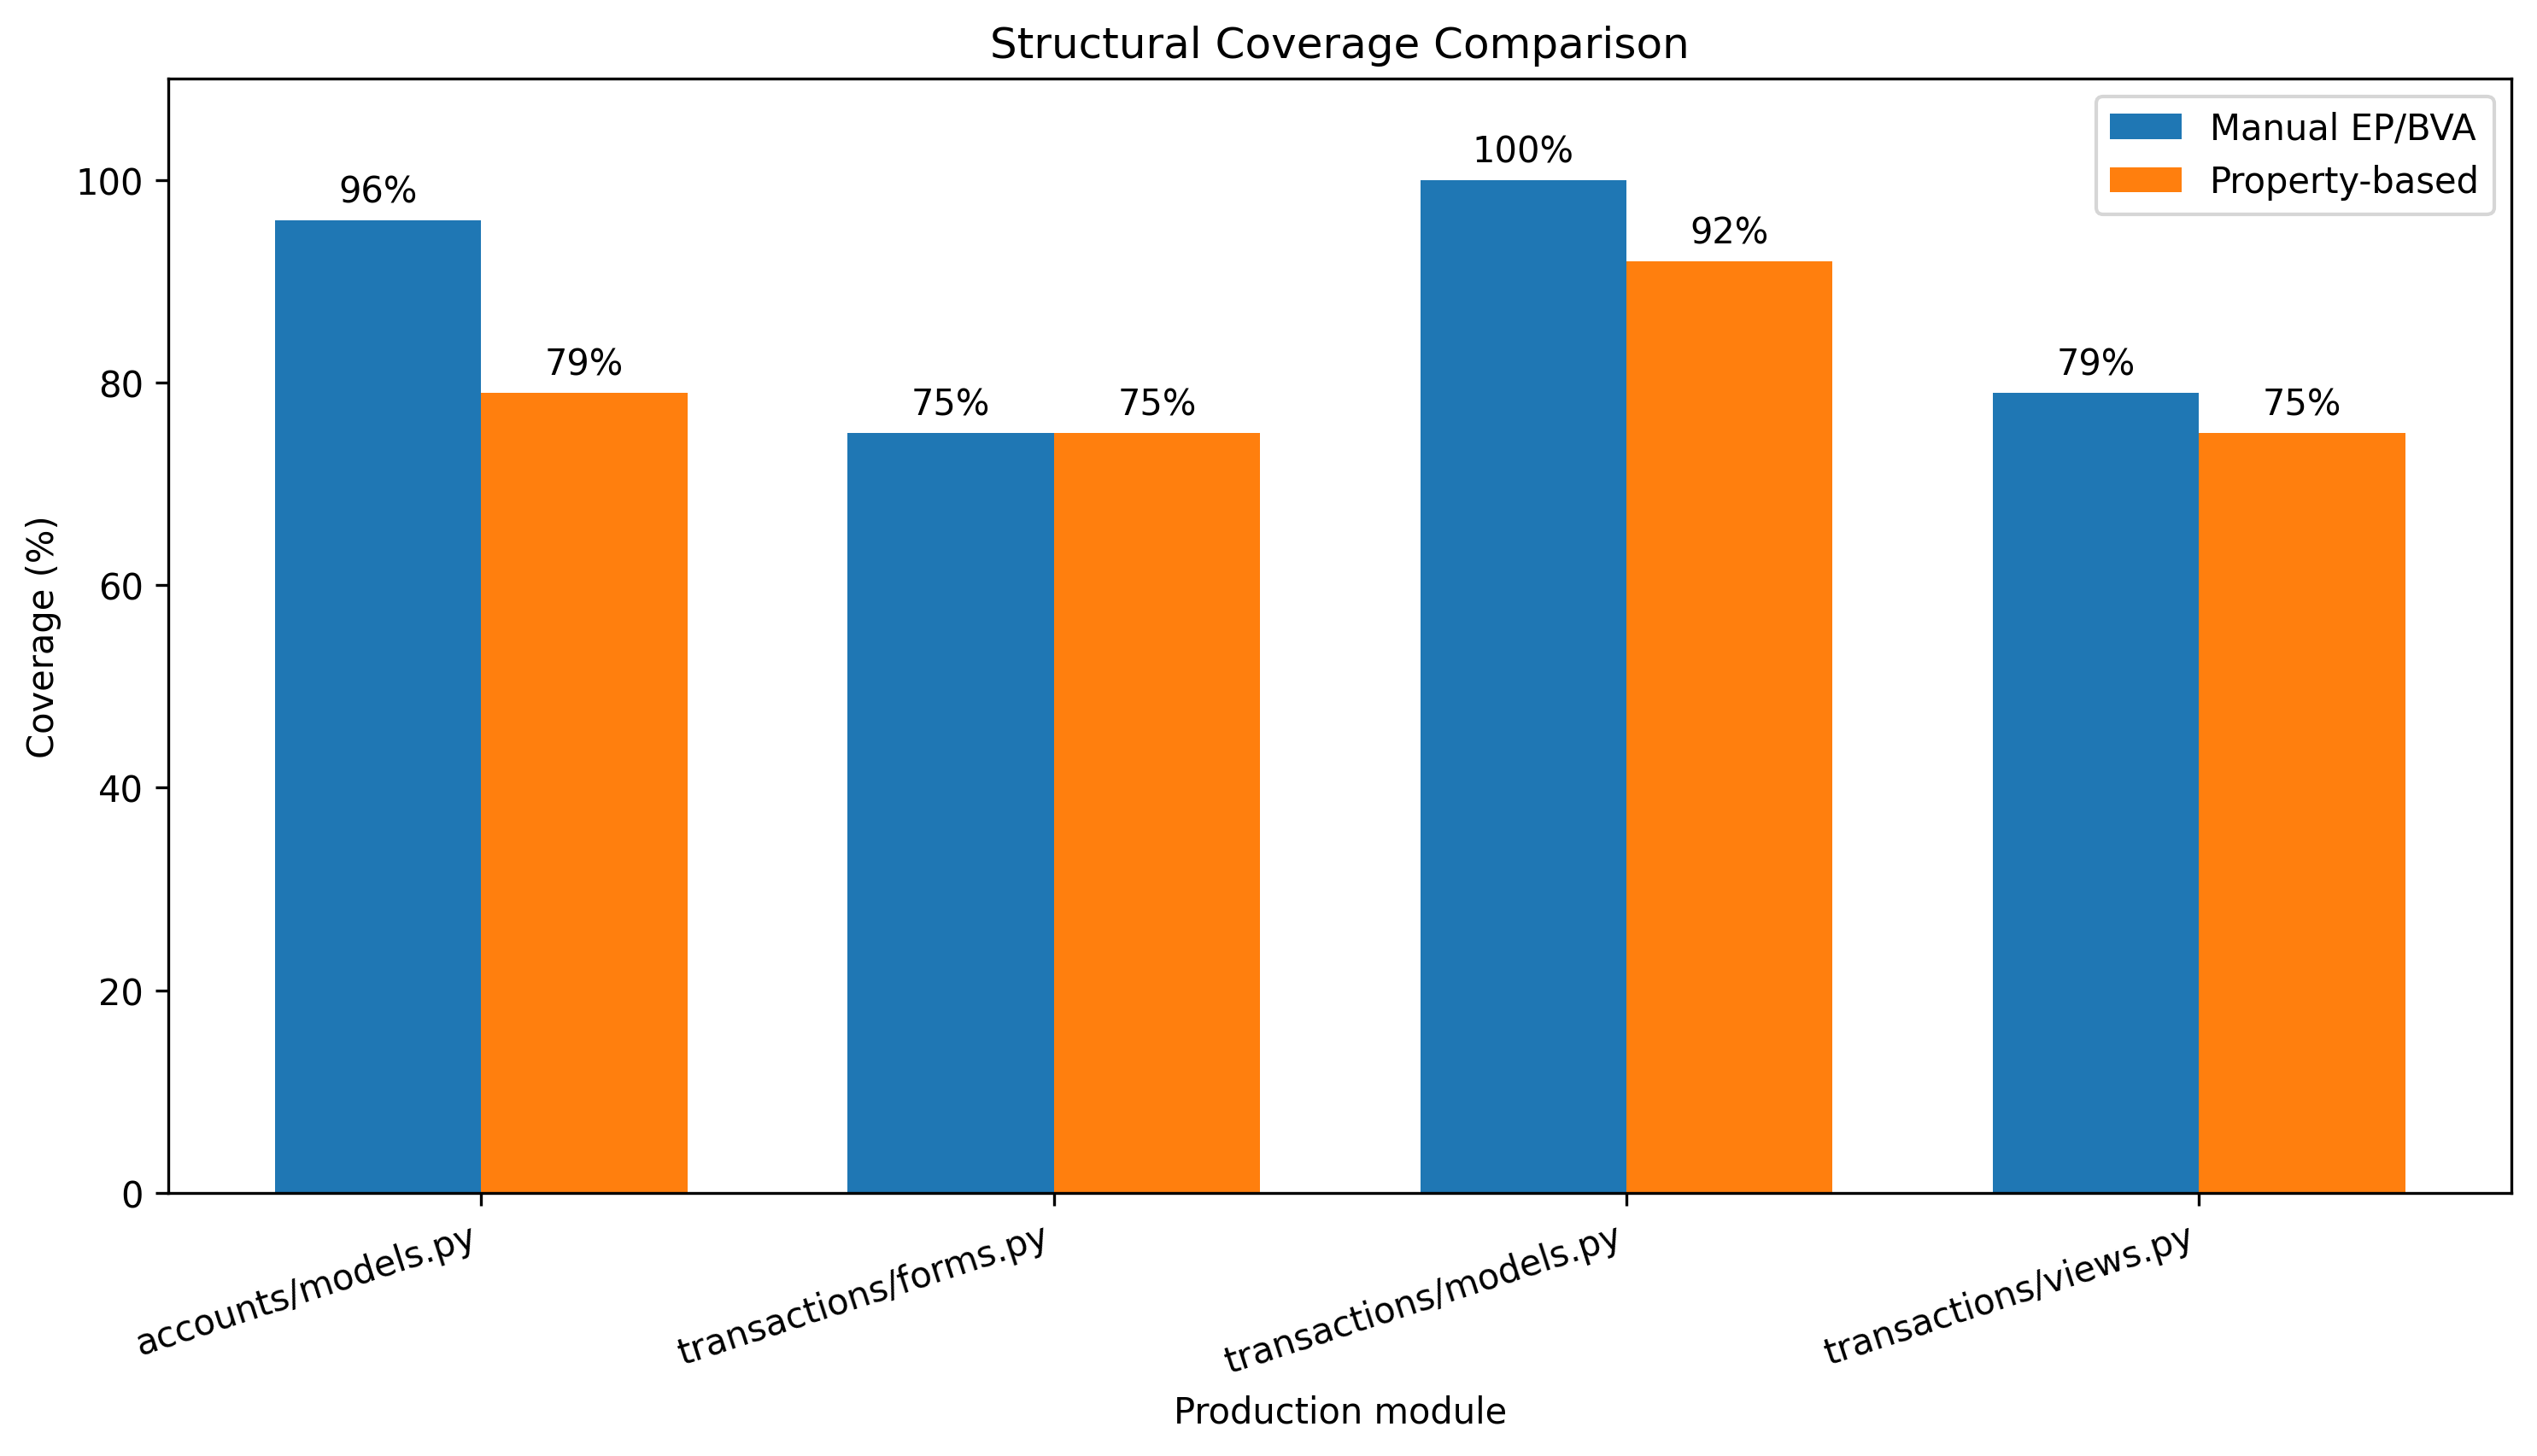
\includegraphics[width=0.90\textwidth]
    {figures/coverage_comparison.png}
    \caption{Structural coverage achieved by the manual and property-based
    test suites for each selected production module.}
    \label{fig:coverage-comparison}
\end{figure}

As shown in Figure~\ref{fig:coverage-comparison}, the manual suite achieved
equal or higher coverage for every selected module. The largest difference
occurred in \texttt{accounts/models.py}, where the manual suite achieved
96\% coverage compared with 79\% for the property-based suite.

% =========================================================
% Mutation Testing Results
% =========================================================

\section{Mutation Testing Results}

\subsection{Generated Mutant Population}

Mutation testing was executed separately for the manual and property-based
test suites using the same production-code scope and the same mutation
configuration.

Each run generated 96 mutants from the same pinned source revision and
identical mutation configuration. The matching counts, target files, and
configuration provide evidence that the mutant population remained consistent
between runs.

\begin{table}[H]
\centering
\caption{Mutation-testing outcome summary}
\label{tab:mutation-summary}
\footnotesize
\setlength{\tabcolsep}{3.5pt}

\begin{tabular}{|p{3.5cm}|c|c|c|c|c|}
\hline
\textbf{Test suite} &
\textbf{Generated} &
\textbf{Killed} &
\textbf{Survived} &
\textbf{No tests} &
\textbf{Timeout} \\
\hline
Manual EP/BVA suite & 96 & 53 & 17 & 26 & 0 \\
\hline
Property-based suite & 96 & 42 & 15 & 39 & 0 \\
\hline
\end{tabular}

\setlength{\tabcolsep}{6pt}
\end{table}

The manual suite killed 53 mutants, while the property-based suite killed 42.
The property-based suite also produced a larger number of no-test outcomes,
indicating that more mutated behaviours were outside its execution reach.

No timeout mutants occurred in either run.

\subsection{Raw Mutation Outcomes}

The raw outcome percentages were calculated relative to the complete
population of 96 mutants.

For the manual suite:

\begin{align}
\text{Killed proportion}
&=
\frac{53}{96}\times 100
=
55.21\% \\
\text{Survived proportion}
&=
\frac{17}{96}\times 100
=
17.71\% \\
\text{No-test proportion}
&=
\frac{26}{96}\times 100
=
27.08\%
\end{align}

For the property-based suite:

\begin{align}
\text{Killed proportion}
&=
\frac{42}{96}\times 100
=
43.75\% \\
\text{Survived proportion}
&=
\frac{15}{96}\times 100
=
15.63\% \\
\text{No-test proportion}
&=
\frac{39}{96}\times 100
=
40.63\%
\end{align}

These raw percentages are useful for describing the complete tool output.
However, they are not the final controlled mutation scores because the
generated population included 26 mutants from a feature that was declared
outside the experiment scope.

\subsection{Controlled Relevant Mutant Population}

The 26 mutants associated with
\texttt{TransactionDateRangeForm.clean\_daterange} were outside the selected
financial transaction scope.

These mutants were classified as no tests in both experimental runs. They were
therefore excluded consistently from the controlled comparison.

The relevant population was:

\begin{equation}
M_{\text{relevant}}
=
96-26
=
70
\end{equation}

For the manual suite, all 70 relevant mutants were reached:

\begin{equation}
53+17=70
\end{equation}

For the property-based suite, 57 relevant mutants were reached and 13 relevant
mutants were classified as no tests:

\begin{equation}
42+15+13=70
\end{equation}

\subsection{Controlled Mutation Scores}

The controlled mutation score used the same denominator of 70 relevant mutants
for both suites.

For the manual suite:

\begin{equation}
MS_{\text{manual}}
=
\frac{53}{70}\times 100
=
75.71\%
\end{equation}

For the property-based suite:

\begin{equation}
MS_{\text{property}}
=
\frac{42}{70}\times 100
=
60.00\%
\end{equation}

The difference was:

\begin{equation}
75.71\%-60.00\%
=
15.71
\text{ percentage points}
\end{equation}

\begin{table}[H]
\centering
\caption{Controlled mutation-score comparison}
\label{tab:controlled-mutation-score}
\footnotesize
\setlength{\tabcolsep}{4pt}

\begin{tabular}{|p{4.2cm}|p{3.2cm}|p{2.8cm}|p{2.6cm}|}
\hline
\textbf{Test suite} &
\textbf{Killed relevant mutants} &
\textbf{Relevant population} &
\textbf{Controlled score} \\
\hline

Manual EP/BVA suite &
53 &
70 &
75.71\% \\
\hline

Property-based suite &
42 &
70 &
60.00\% \\
\hline

\end{tabular}

\setlength{\tabcolsep}{6pt}
\end{table}

Under this controlled interpretation, the manual suite achieved the higher
mutation score.

\subsection{Reached-Mutant Scores}

The controlled score combines two factors:

\begin{itemize}
    \item whether the suite reaches the mutated behaviour; and
    \item whether its oracle detects the behavioural change.
\end{itemize}

To examine oracle effectiveness within reached code, a second score was
calculated using only killed and surviving mutants.

For the manual suite:

\begin{equation}
MS_{\text{manual,reached}}
=
\frac{53}{53+17}\times 100
=
75.71\%
\end{equation}

For the property-based suite:

\begin{equation}
MS_{\text{property,reached}}
=
\frac{42}{42+15}\times 100
=
73.68\%
\end{equation}

\begin{table}[H]
\centering
\caption{Reached-mutant mutation-score comparison}
\label{tab:reached-mutation-score}

\begin{tabular}{|p{5cm}|c|c|c|}
\hline
\textbf{Test suite} &
\textbf{Killed} &
\textbf{Survived} &
\textbf{Reached-mutant score} \\
\hline

Manual EP/BVA suite &
53 &
17 &
75.71\% \\
\hline

Property-based suite &
42 &
15 &
73.68\% \\
\hline

\end{tabular}
\end{table}

The reached-mutant scores differed by only 2.03 percentage points. This is
substantially smaller than the 15.71-point difference observed using the
controlled relevant population.

This result suggests that the main difference between the suites was
behavioural reach. Once mutated code was reached, their fault-detection
effectiveness was relatively similar.

\begin{figure}[H]
    \centering
    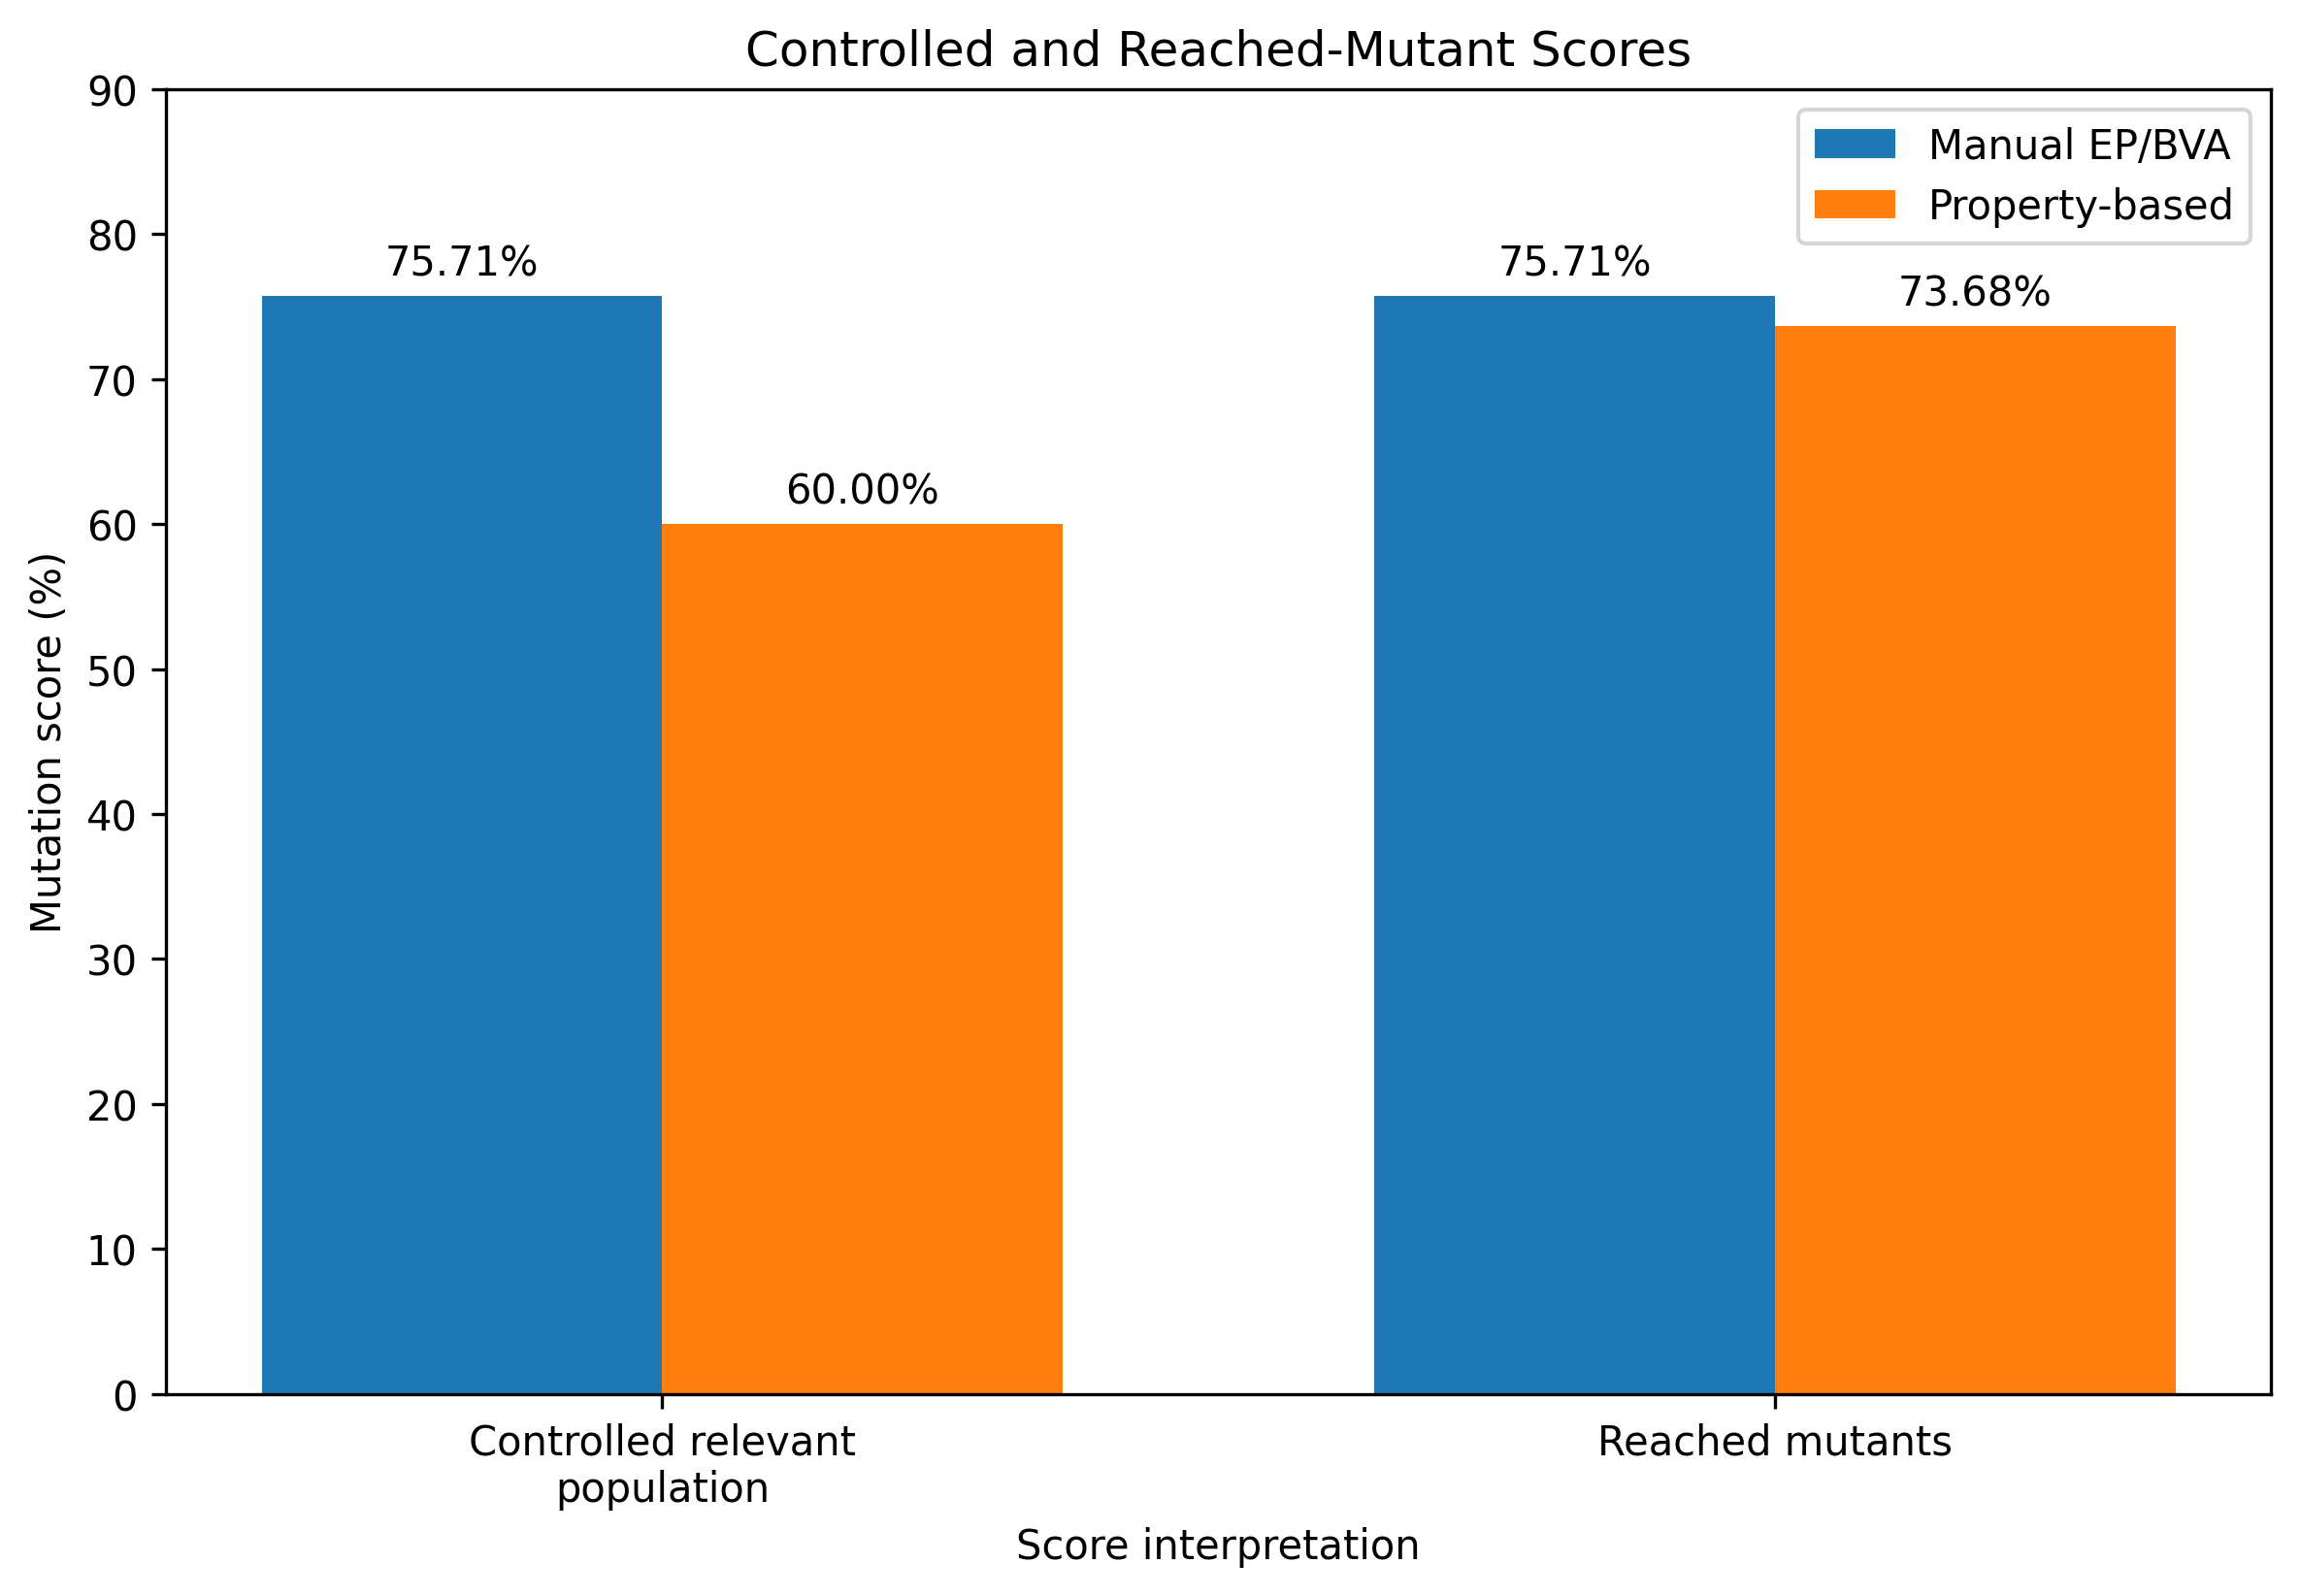
\includegraphics[width=0.82\textwidth]
    {figures/mutation_score_comparison.png}
    \caption{Comparison of controlled relevant-population and reached-mutant
    mutation scores.}
    \label{fig:mutation-score-comparison}
\end{figure}

Figure~\ref{fig:mutation-score-comparison} shows that the controlled scores
differed by 15.71 percentage points, while the reached-mutant scores differed
by only 2.03 percentage points. This supports the conclusion that behavioural
reach was the principal source of the overall difference.

\subsection{Interpretation of No-Test Outcomes}

The manual suite produced 26 no-test mutants, all of which belonged to the
known out-of-scope date-range form.

The property-based suite produced 39 no-test mutants. After removing the same
26 out-of-scope mutants, 13 relevant mutants remained untested.

These additional no-test outcomes are consistent with the narrower property
catalogue and the lower structural coverage observed in
\texttt{accounts/models.py}, \texttt{transactions/models.py}, and
\texttt{transactions/views.py}.

The no-test classification should not be interpreted as an assertion failure.
It indicates that the selected suite did not execute the mutated code.

\subsection{Mutation Result Artifacts}

The complete mutation outputs were preserved under:

\begin{verbatim}
results/mutation/manual/
results/mutation/property_based/
\end{verbatim}

Each directory contains:

\begin{itemize}
    \item the complete mutant result list;
    \item the summary output;
    \item surviving-mutant identifiers;
    \item setup information; and
    \item exported survivor details.
\end{itemize}

A consolidated comparison was stored in:

\begin{verbatim}
results/mutation/comparison_summary.txt
\end{verbatim}

\subsection{Mutation Outcome Comparison}

Figure~\ref{fig:mutation-outcomes} compares the raw mutation outcomes for the
manual and property-based test suites across the consistently generated
population of 96 mutants.

\begin{figure}[H]
    \centering
    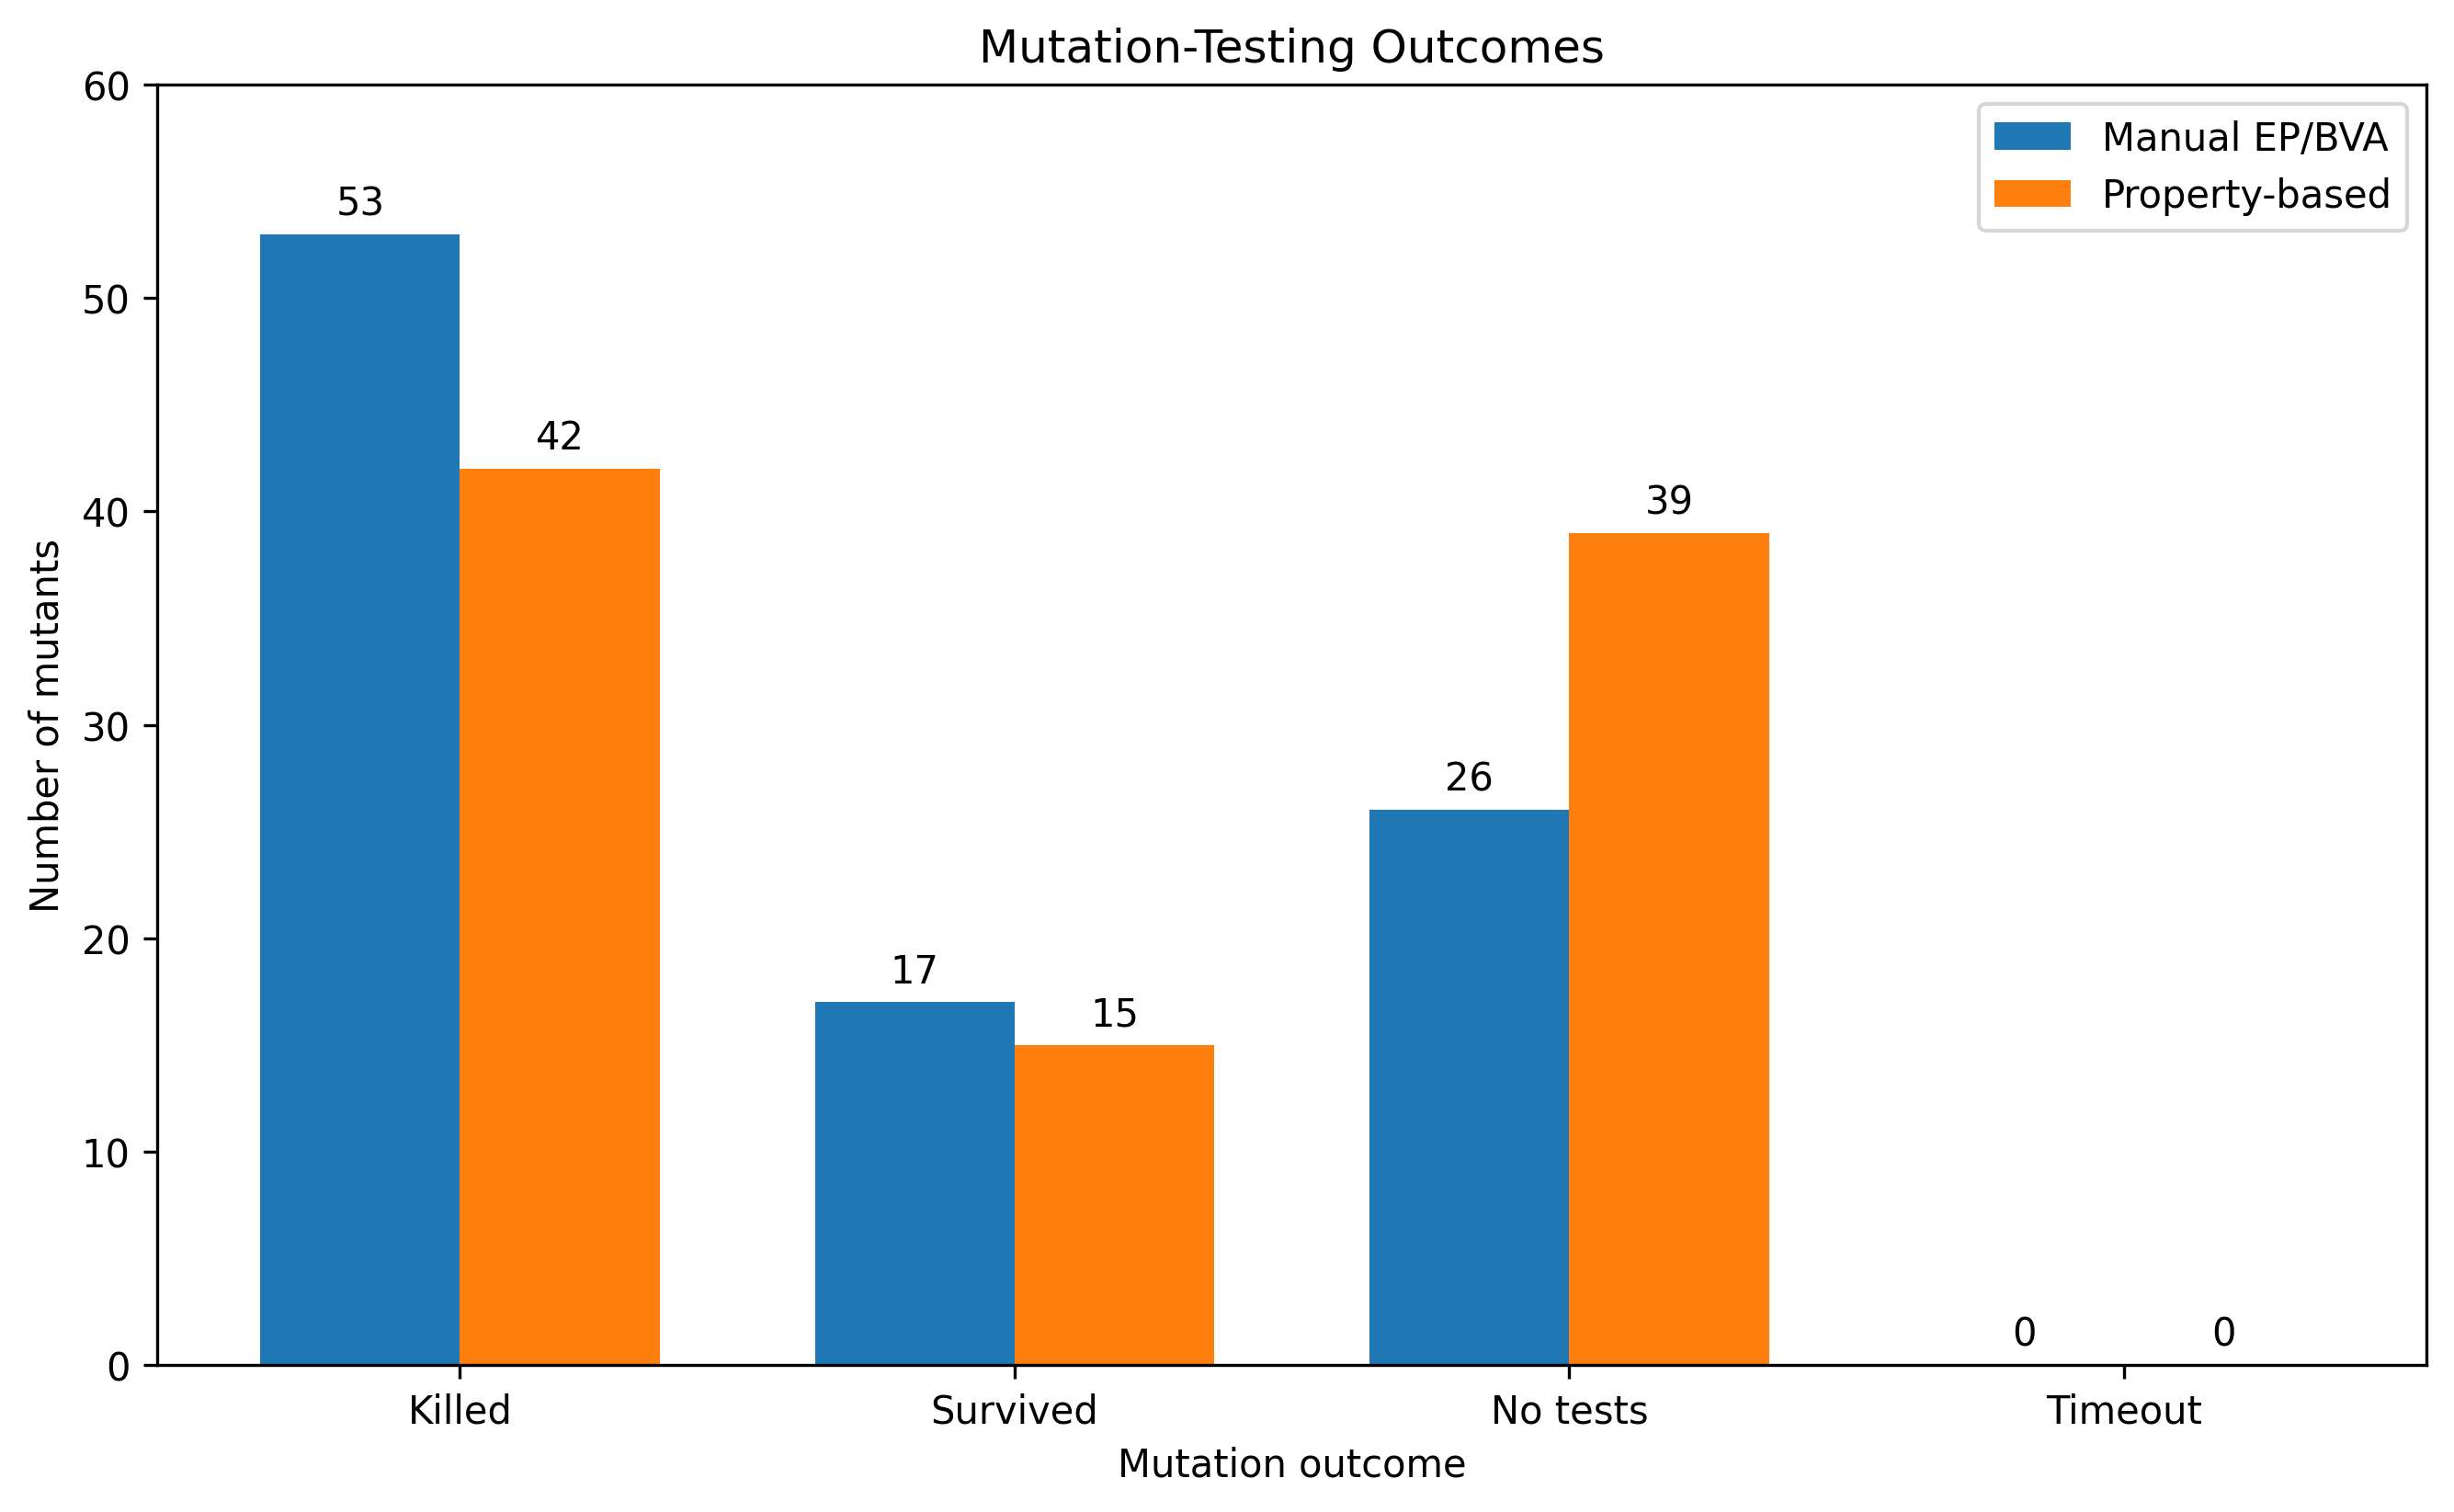
\includegraphics[width=0.88\textwidth]
    {figures/mutation_outcomes.png}
    \caption{Mutation-testing outcomes for the manual and property-based
    test suites.}
    \label{fig:mutation-outcomes}
\end{figure}

As shown in Figure~\ref{fig:mutation-outcomes}, the manual suite killed more
mutants and produced fewer no-test outcomes. The manual suite killed 53
mutants and produced 26 no-test outcomes, whereas the property-based suite
killed 42 mutants and produced 39 no-test outcomes. This result supports the
interpretation that the manual suite reached a broader portion of the selected
behavioural scope.

% =========================================================
% Surviving-Mutant Analysis
% =========================================================

\section{Surviving-Mutant Analysis}

\subsection{Purpose of Survivor Analysis}

Mutation score alone does not explain why mutants survive. A surviving mutant
may indicate a genuine weakness in the test suite, an equivalent change, an
underspecified requirement, or behaviour outside the study scope.

For this reason, the surviving mutants were inspected individually. The manual
suite produced 17 unique survivors, and each was classified according to its
semantic effect and relationship to the reconstructed requirements.

\subsection{Survivor Classification}

The 17 manual-suite survivors were classified as follows:

\begin{table}[H]
\centering
\caption{Classification of unique surviving mutants}
\label{tab:survivor-classification}
\footnotesize
\setlength{\tabcolsep}{4pt}

\begin{tabular}{|p{5.4cm}|c|p{7.2cm}|}
\hline
\textbf{Classification} &
\textbf{Count} &
\textbf{Interpretation} \\
\hline

Genuine test weakness &
7 &
The mutant changed financially relevant behaviour, but the existing tests did
not detect the change. \\
\hline

Equivalent or likely equivalent &
2 &
The source change did not appear to alter observable behaviour for the valid
input domain considered in the study. \\
\hline

Underspecified diagnostic text &
7 &
The mutant altered validation-message wording or formatting, while the
financial acceptance or rejection behaviour remained unchanged. \\
\hline

Outside core scope &
1 &
The mutant affected behaviour that was not part of the principal financial
verification objective. \\
\hline

\textbf{Total} &
\textbf{17} &
\\
\hline

\end{tabular}

\setlength{\tabcolsep}{6pt}
\end{table}

The classification shows that fewer than half of the survivors represented
clear financial test weaknesses. Several survived because the study
intentionally did not specify exact diagnostic text.

\subsection{Genuine Test Weaknesses}

Seven survivors were classified as genuine weaknesses. These mutants were
concentrated in four areas:

\begin{itemize}
    \item interest arithmetic;
    \item monetary rounding;
    \item interest-calculation scheduling; and
    \item positional form initialization.
\end{itemize}

\subsubsection{Interest Arithmetic}

Some mutants changed arithmetic used in the interest calculation. These
survivors showed that the existing tests did not distinguish all relevant
operator or constant substitutions.

A general interest oracle was present, but certain generated or fixed examples
did not make the mutated and original expressions sufficiently different.
This demonstrates that a mathematically meaningful property can still be too
weak when the selected input domain does not expose the change.

A stronger test design would include independently calculated expected values
for several combinations of principal, rate, and calculation frequency.

\subsubsection{Monetary Rounding}

Mutants affecting rounding behaviour also survived. Financial software should
handle currency precision explicitly, since small rounding differences may
accumulate or produce inconsistent recorded balances.

The existing tests checked two-decimal output in some cases, but they did not
include enough values near rounding boundaries.

Additional examples should include values whose third decimal digit is:

\begin{itemize}
    \item below five;
    \item exactly five; and
    \item above five.
\end{itemize}

This would increase sensitivity to mutations affecting rounding precision or
rounding position.

\subsubsection{Interest-Calculation Scheduling}

The manual suite included explicit examples for interest-calculation month
scheduling. However, the selected assertions did not distinguish every mutated
variation of the scheduling logic. This demonstrates that executing a helper
method and checking selected outputs may still leave alternative mutated
schedules observationally equivalent for the chosen examples.

The property-based suite did not directly represent this behaviour in its
original property catalogue. This omission also contributed to its reduced
reach within \texttt{accounts/models.py}.

A stronger oracle would verify:

\begin{itemize}
    \item the exact number of calculated months;
    \item the first expected month;
    \item the interval between successive months;
    \item the absence of duplicates; and
    \item valid month values between 1 and 12.
\end{itemize}

\subsubsection{Positional Form Initialization}

One surviving mutant affected positional initialization behaviour in a
transaction form. The original tests primarily constructed the form using
keyword arguments.

As a result, a mutation affecting positional argument handling was not
detected. A dedicated test should instantiate the form using the supported
positional calling pattern and verify that account and transaction-type
information are assigned correctly.

\subsection{Equivalent or Likely Equivalent Mutants}

Two survivors were classified as equivalent or likely equivalent.

Equivalent mutants are syntactically different from the original program but
produce the same observable behaviour for all relevant inputs. Such mutants
cannot be killed by adding a valid test unless the specification is changed.

Because proving semantic equivalence is generally difficult, these mutants
were classified conservatively as likely equivalent based on source inspection
and repeated execution over the relevant input domain.

They were retained in the raw tool output but distinguished from genuine test
weaknesses during interpretation.

\subsection{Underspecified Diagnostic-Text Mutants}

Seven survivors altered validation-message text without changing the financial
decision.

For example, a mutant may change capitalization, punctuation, or wording while
the same invalid transaction is still rejected.

The reconstructed requirements specified whether an input must be accepted or
rejected, but they did not define exact diagnostic strings. Therefore, tests
that assert only validation failure are consistent with the specification.

These survivors do not demonstrate incorrect financial behaviour. Instead,
they expose underspecified presentation-level behaviour.

Requiring exact message text would increase the mutation score, but it would
also make the suite more brittle and more tightly coupled to user-interface
wording.

\subsection{Outside-Scope Survivor}

One survivor affected behaviour outside the principal financial verification
scope.

This mutant was documented but was not treated as evidence of weakness in the
core deposit, withdrawal, balance, transaction, or interest requirements.

\subsection{Manual and Property Survivor Relationship}

The manual suite produced 17 survivors, while the property-based suite produced
15. These counts alone should not be used to conclude that the property suite
was stronger.

The property suite reached only 57 of the 70 relevant mutants. Therefore, some
mutants that survived under the manual suite may have been classified as no
tests under the property suite rather than as killed.

The reached-mutant scores provide a fairer comparison of oracle effectiveness:

\[
MS_{\text{manual,reached}} = 75.71\%
\]

\[
MS_{\text{property,reached}} = 73.68\%
\]

These close scores indicate that the principal difference was reach rather than
a large difference in detection strength within executed behaviour.

\subsection{Lessons from Survivor Analysis}

The survivor analysis produced four important lessons.

First, broad code execution does not guarantee strong test oracles. Some
financial arithmetic was reached, but the existing assertions did not
distinguish the original implementation from the mutated version.

Second, property-based testing depends on the completeness of the property
catalogue. Generating many inputs cannot compensate for an omitted behaviour
or helper method.

Third, exact validation-message assertions should be introduced only when the
message wording is explicitly part of the specification. Otherwise, such tests
may increase brittleness without improving verification of financial
correctness.

Fourth, mutation results are more informative when surviving mutants are
examined semantically rather than reported only as a percentage. Survivor
classification helps distinguish genuine test weaknesses from equivalent,
underspecified, or out-of-scope behaviour.

\subsection{Survivor Analysis Artifact}

The complete survivor analysis was preserved in:

\begin{verbatim}
docs/surviving_mutant_analysis.md
\end{verbatim}

Detailed source-level mutant information was also exported as follows:

\begin{verbatim}
results/mutation/survivor_details/
\end{verbatim}

These artifacts record the mutant location, source change, classification, and
recommended test improvement.

% =========================================================
% Discussion
% =========================================================

\section{Discussion}

\subsection{Answer to the Primary Research Question}

The primary research question asked how the mutation adequacy of a manually
designed equivalence-partitioning and boundary-value suite compared with that
of a Hypothesis property-based suite for the selected financial subsystem.

Using the controlled population of 70 relevant mutants, the manual suite
achieved a mutation score of 75.71\%, while the property-based suite achieved
60.00\%. The manual suite therefore achieved the higher controlled mutation
score by 15.71 percentage points.

This result does not mean that manually designed testing is universally more
effective than property-based testing. In this experiment, the manual suite
represented a broader range of account, transaction, and helper behaviours.
The property-based suite focused more narrowly on the principal financial
invariants.

When only reached mutants were considered, the difference was much smaller.
The manual suite achieved 75.71\%, while the property-based suite achieved
73.68\%. This 2.03-point difference indicates that the two suites had similar
fault-detection effectiveness within the code they actually exercised.

The main experimental difference was therefore behavioural reach rather than
a large difference in oracle strength.

\subsection{RQ1: Which Suite Achieved Higher Structural Coverage?}

The manual suite achieved higher overall structural coverage.

\begin{itemize}
    \item Manual suite: 84\%.
    \item Property-based suite: 77\%.
    \item Difference: 7 percentage points.
\end{itemize}

The largest module-level difference occurred in
\texttt{accounts/models.py}, where the manual suite achieved 96\% coverage and
the property-based suite achieved 79\%.

The manual suite also achieved higher coverage in
\texttt{transactions/models.py} and \texttt{transactions/views.py}. Both
suites achieved 75\% in \texttt{transactions/forms.py}.

These results support the conclusion that the manual suite represented a
broader portion of the selected subsystem.

\subsection{RQ2: Which Suite Reached a Broader Range of Financial Behaviour?}

The mutation no-test outcomes provide direct evidence about behavioural reach.

After excluding the 26 common out-of-scope mutants, the manual suite reached
all 70 relevant mutants. The property-based suite reached 57 and did not reach
13 relevant mutants.

The property-based suite's lower reach was mainly associated with behaviours
that were absent from its property catalogue, including selected account-model
and helper functionality.

This result illustrates an important limitation of property-based testing:
automatic generation can explore many values only within the behaviours that
have been encoded as properties. It does not automatically discover missing
requirements or omitted helper methods.

\subsection{RQ3: Which Categories of Mutants Survived?}

The surviving mutants fell into four principal categories:

\begin{enumerate}
    \item genuine financial test weaknesses;
    \item equivalent or likely equivalent changes;
    \item underspecified diagnostic-message changes; and
    \item behaviour outside the principal scope.
\end{enumerate}

The genuine weaknesses were concentrated in interest arithmetic, monetary
rounding, interest-calculation scheduling, and positional form initialization.

The diagnostic-message survivors show that mutation testing can reveal
underspecified requirements as well as weak tests. The tests correctly checked
financial rejection behaviour, but they did not require exact wording because
the specification did not define it.

\subsection{RQ4: What Relationship Was Observed Between Coverage and Mutation
Adequacy?}

The manual suite achieved both higher structural coverage and a higher
controlled mutation score.

However, the relationship was not one-to-one. The overall coverage difference
was 7 percentage points, while the controlled mutation-score difference was
15.71 percentage points.

This occurred because mutation score reflects both execution and detection.
Coverage measures whether code is executed, while mutation testing also checks
whether assertions distinguish the original behaviour from a modified version.

The reached-mutant scores were close even though the overall coverage values
differed. This further supports the interpretation that the manual suite's
main advantage was broader reach.

\subsection{Manual EP/BVA Strengths}

The manual suite had several strengths.

First, the explicit requirements-to-test traceability encouraged broad
representation of the subsystem.

Second, equivalence partitioning ensured that valid and invalid classes were
considered systematically.

Third, boundary value analysis directly targeted financial thresholds such as
minimum deposit, minimum withdrawal, maximum withdrawal, and available
balance.

Fourth, fixed examples supported precise arithmetic and persistence assertions.

These strengths contributed to the suite's broader structural and mutation
reach.

\subsection{Manual EP/BVA Limitations}

The manual approach depended strongly on tester judgement.

A partition, boundary, or helper behaviour could be missed if it was not
identified during design. Fixed examples may also fail to expose faults that
occur only for unusual numeric combinations.

Manual tests can therefore provide strong traceability and breadth, but their
input diversity remains limited unless many examples are added.

\subsection{Property-Based Testing Strengths}

The property-based suite expressed financial behaviour in a reusable and
general form.

Generated values allowed the same invariant to be evaluated across many
inputs. Relational properties such as exact balance change and monotonicity
were natural to express using Hypothesis.

Shrinking also improved failure diagnosis by reducing complex failing examples
to simpler counterexamples.

Within reached code, the property-based suite achieved a reached-mutant score
close to that of the manual suite. This indicates that its financial
properties were generally effective when they exercised the relevant
behaviour.

\subsection{Property-Based Testing Limitations}

The main limitation was catalogue completeness.

The property suite did not directly represent every selected account and
transaction helper. As a result, 13 relevant mutants were not reached.

Some properties may also be too general to detect particular arithmetic or
rounding mutations. A property such as non-negativity can pass even when the
computed value is financially incorrect.

Property-based testing therefore requires both strong invariants and broad
behavioural traceability.

\subsection{Complementary Use of Both Approaches}

The results support treating the two approaches as complementary rather than
as substitutes.

Manual EP/BVA testing is effective for:

\begin{itemize}
    \item explicit requirement traceability;
    \item known input partitions;
    \item threshold-focused validation;
    \item helper-method coverage; and
    \item precise expected-value examples.
\end{itemize}

Property-based testing is effective for:

\begin{itemize}
    \item exploring many values within defined domains;
    \item checking general invariants;
    \item finding unexpected numeric combinations;
    \item testing relational properties; and
    \item minimizing counterexamples through shrinking.
\end{itemize}

A stronger combined strategy would use EP/BVA to ensure behavioural breadth
and Hypothesis to deepen exploration within each identified requirement.

\subsection{Implications for Financial Software Testing}

Financial software requires more than successful execution. Tests should verify
exact monetary effects, state preservation, persistence consistency, and
rounding behaviour.

The survivor analysis showed that weak arithmetic or precision checks can
allow financially significant mutations to survive. It also showed that
broadly stated properties may not be sufficient unless they are paired with
independent expected-value calculations.

For financial systems, a robust suite should therefore include:

\begin{itemize}
    \item explicit boundary cases;
    \item generated valid and invalid amounts;
    \item exact before-and-after balance assertions;
    \item independent arithmetic oracles;
    \item rounding-boundary examples;
    \item persistence checks; and
    \item mutation analysis to evaluate oracle strength.
\end{itemize}

\subsection{Overall Interpretation}

The study does not establish that one test-design technique is always superior.

For this subject system and experimental scope, the manual suite achieved
better overall adequacy because it covered a broader set of behaviours. The
property-based suite was nearly as effective within reached code, but its
property catalogue was narrower.

The most defensible conclusion is therefore:

\begin{quote}
Manual EP/BVA testing provided broader behavioural coverage in this case
study, while property-based testing provided comparable fault-detection
strength within the behaviours it exercised. The strongest practical strategy
is to combine explicit requirement-based breadth with generated
property-based depth.
\end{quote}

% =========================================================
% Threats to Validity
% =========================================================

\section{Threats to Validity}

\subsection{Internal Validity}

Internal validity concerns whether the observed differences were caused by the
test-design approaches rather than by uncontrolled experimental factors.

Several controls were applied. Both suites were executed against the same
pinned source revision, the same selected production modules, the same Python
environment, the same database setup, and the same mutation tool. Both mutation
runs generated 96 mutants, providing evidence that the mutant population was
stable.

However, some internal-validity threats remain.

First, the two suites were not equal in behavioural breadth. The manual suite
explicitly covered more helper methods, while the property-based suite focused
on a narrower property catalogue. Therefore, the experiment compares the
implemented suites as designed, not two perfectly size-matched or
scope-matched artifacts.

Second, manual judgement influenced both requirement extraction and survivor
classification. Another tester might identify different equivalence classes,
write different properties, or classify ambiguous mutants differently.

Third, the tests were created with knowledge of the implementation structure.
Although the manual suite was based on EP/BVA and the property suite was based
on invariants, source inspection was required to reconstruct requirements and
configure the experiment. This may have influenced test selection.

\subsection{Construct Validity}

Construct validity concerns whether the selected measurements accurately
represent test adequacy.

Structural coverage was measured using statement and branch coverage. These
metrics indicate execution but do not directly measure oracle strength.

Mutation score was therefore used as the principal adequacy measure. However,
mutation testing is only a proxy for real fault detection. The generated
mutants may not fully represent realistic financial defects.

Equivalent and underspecified mutants also affect interpretation. A surviving
mutant may not indicate a test weakness when the modified program is
semantically equivalent or when the changed behaviour is not part of the
requirements.

To reduce this threat, raw mutation outcomes, controlled mutation scores,
reached-mutant scores, and semantic survivor classifications were reported
separately.

\subsection{External Validity}

External validity concerns whether the findings generalize beyond this case
study.

The experiment used one open-source Django banking application and one selected
financial subsystem. The findings may not generalize directly to other
applications, programming languages, frameworks, domains, or mutation tools.

The subject system also lacked a direct inter-account transfer feature.
Therefore, traditional transfer-conservation properties were replaced with
deposit, withdrawal, and state-preservation invariants.

The relative performance of manual and property-based testing may differ in a
system with more complex calculations, concurrency, distributed transactions,
or a larger existing test suite.

Accordingly, the conclusions are limited to this subject system, source
revision, toolchain, and declared scope.

\subsection{Conclusion Validity}

Conclusion validity concerns whether the numerical evidence supports the
reported interpretation.

The experiment used one execution configuration and one pair of test suites.
No statistical hypothesis test was performed because the primary data
consisted of deterministic coverage and mutation outcomes for a single pinned
revision.

The controlled mutation-score difference was 15.71 percentage points, while
the reached-mutant difference was only 2.03 percentage points. This distinction
was important for avoiding an overly broad conclusion that the manual suite
had much stronger assertions.

The results support the narrower conclusion that the manual suite had broader
behavioural reach, while the two suites had similar effectiveness within
reached code.

\subsection{Reliability and Reproducibility}

Reliability concerns whether another investigator could repeat the experiment
and obtain comparable results.

The project improves repeatability by preserving:

\begin{itemize}
    \item the pinned upstream revision;
    \item dependency versions;
    \item separate test-suite directories;
    \item coverage commands and reports;
    \item mutation setup scripts;
    \item raw mutation outputs;
    \item exported survivor details; and
    \item the survivor-classification document.
\end{itemize}

Despite these controls, exact reproduction may still depend on operating-system
behaviour, dependency availability, database configuration, or future changes
in external tools.

\subsection{Researcher Bias}

The same researcher designed the tests, executed the experiment, interpreted
the outputs, and classified surviving mutants. This creates a risk of
confirmation bias.

To reduce this risk, classifications were based on explicit criteria:

\begin{itemize}
    \item whether the mutant changed observable financial behaviour;
    \item whether the behaviour was included in the declared requirements;
    \item whether the suite reached the mutated code;
    \item whether the existing oracle could observe the change; and
    \item whether the mutant appeared equivalent for the relevant input
          domain.
\end{itemize}

The detailed mutant artifacts were retained so that the classifications can be
reviewed independently.

\subsection{Mitigation Summary}

The principal mitigation measures were:

\begin{itemize}
    \item identical source and mutation scope for both suites;
    \item a stable generated mutant population;
    \item separate execution of each suite;
    \item explicit requirements and invariants;
    \item preservation of raw artifacts;
    \item separate reporting of raw, controlled, and reached-mutant results;
    \item semantic survivor inspection; and
    \item cautious limitation of the final conclusions.
\end{itemize}

These measures do not eliminate all threats, but they make the experimental
assumptions and limitations visible.

% =========================================================
% Reproduction Instructions and Practical Artifacts
% =========================================================

\section{Reproduction Instructions and Practical Artifact}

\subsection{Artifact Overview}

The practical artifact contains the subject system, both test suites,
requirements and invariant documents, coverage reports, mutation outputs,
surviving-mutant details, and automation scripts.

The repository is available at:

\begin{center}
\url{https://github.com/hadiChowdhury/Svv-banking-verification-study}
\end{center}

The principal repository structure is:

\begin{verbatim}
Svv-banking-verification-study/
|-- subject_system/
|   `-- banking_system/
|-- tests/
|   |-- manual/
|   `-- property_based/
|-- docs/
|-- results/
|   |-- coverage/
|   `-- mutation/
|-- scripts/
|-- requirements.txt
|-- pytest.ini
`-- README.md
\end{verbatim}

\subsection{Prerequisites}

The experiment requires:

\begin{itemize}
    \item Python 3.10;
    \item Git;
    \item a command-line terminal; and
    \item the dependencies listed in \texttt{requirements.txt}.
\end{itemize}

The experiment was originally executed using Python 3.10.20. Using the same
major and minor Python version is recommended because the subject system uses
an older Django release.

\subsection{Repository Setup}

Clone the repository and enter the project directory:

\begin{lstlisting}[language=bash,caption={Cloning the project repository}]
git clone https://github.com/hadiChowdhury/Svv-banking-verification-study.git
cd Svv-banking-verification-study
\end{lstlisting}

Create a virtual environment:

\begin{lstlisting}[language=bash,caption={Creating a Python virtual environment}]
python3.10 -m venv .venv
\end{lstlisting}

Activate it on macOS or Linux:

\begin{lstlisting}[language=bash,caption={Activating the environment on macOS or Linux}]
source .venv/bin/activate
\end{lstlisting}

On Windows PowerShell:

\begin{lstlisting}[language=bash,caption={Activating the environment on Windows}]
.venv\Scripts\Activate.ps1
\end{lstlisting}

Install the dependencies:

\begin{lstlisting}[language=bash,caption={Installing project dependencies}]
python -m pip install --upgrade pip
pip install -r requirements.txt
\end{lstlisting}

\subsection{Executing the Manual Suite}

The manual EP/BVA suite was executed independently using the following
verified command:

\begin{lstlisting}[language=bash,caption={Executing the manual EP/BVA suite}]
pytest -c mutmut_pytest.ini tests/manual -q
\end{lstlisting}

The observed result was:

\begin{verbatim}
29 passed
\end{verbatim}

\subsection{Executing the Property-Based Suite}

The property-based suite was executed independently using the following
verified command:

\begin{lstlisting}[language=bash,caption={Executing the property-based suite}]
pytest -c mutmut_pytest.ini tests/property_based -q
\end{lstlisting}

The observed result was:

\begin{verbatim}
16 passed
\end{verbatim}

A passing Hypothesis test function may execute many generated examples.
Therefore, the reported 16 test functions should not be interpreted as only
16 individual input executions.

\subsection{Collecting Manual-Suite Coverage}

Manual-suite statement and branch coverage were collected using the following
verified command:

\begin{lstlisting}[language=bash,caption={Collecting manual-suite coverage}]
pytest -c mutmut_pytest.ini tests/manual \
  --cov=accounts.models \
  --cov=transactions.forms \
  --cov=transactions.models \
  --cov=transactions.views \
  --cov-branch \
  --cov-report=term-missing
\end{lstlisting}

The run completed with 29 passing tests and produced the following coverage
results:

\begin{itemize}
    \item 96\% for \texttt{accounts/models.py};
    \item 75\% for \texttt{transactions/forms.py};
    \item 100\% for \texttt{transactions/models.py};
    \item 79\% for \texttt{transactions/views.py}; and
    \item 84\% overall.
\end{itemize}

The preserved outputs are available in:

\begin{verbatim}
results/coverage/manual_coverage.txt
results/coverage/manual_coverage.json
\end{verbatim}

\subsection{Collecting Property-Suite Coverage}

Property-based statement and branch coverage were collected using the following
verified command:

\begin{lstlisting}[language=bash,caption={Collecting property-based coverage}]
pytest -c mutmut_pytest.ini tests/property_based \
  --cov=accounts.models \
  --cov=transactions.forms \
  --cov=transactions.models \
  --cov=transactions.views \
  --cov-branch \
  --cov-report=term-missing
\end{lstlisting}

The run completed with 16 passing tests and produced the following coverage
results:

\begin{itemize}
    \item 79\% for \texttt{accounts/models.py};
    \item 75\% for \texttt{transactions/forms.py};
    \item 92\% for \texttt{transactions/models.py};
    \item 75\% for \texttt{transactions/views.py}; and
    \item 77\% overall.
\end{itemize}

The preserved outputs are available in:

\begin{verbatim}
results/coverage/property_coverage.txt
results/coverage/property_coverage.json
\end{verbatim}

\subsection{Preparing the Mutation Workspace}

The repository includes a script for preparing a clean mutation-testing
workspace:

\begin{lstlisting}[language=bash,caption={Preparing the mutation workspace}]
bash scripts/prepare_mutation_workspace.sh
\end{lstlisting}

The mutation configuration must be checked before each run so that the correct
test suite is selected.

The manual mutation run must invoke only the manual suite. The property-based
mutation run must invoke only the property-based suite.

\subsection{Executing the Manual Mutation Run}

The saved manual mutation configuration was restored before creating a clean
mutation workspace:

\begin{lstlisting}[language=bash,caption={Executing the manual mutation run}]
cp results/mutation/manual/setup.cfg setup.cfg
rm -rf mutants
mutmut run
\end{lstlisting}

The observed manual mutation result was:

\begin{verbatim}
Generated: 96
Killed:    53
Survived:  17
No tests:  26
Timeout:    0
\end{verbatim}

\subsection{Executing the Property-Based Mutation Run}

The property-based configuration was restored and the previous mutation
workspace was removed:

\begin{lstlisting}[language=bash,caption={Executing the property-based mutation run}]
cp results/mutation/property_based/setup.cfg setup.cfg
rm -rf mutants
mutmut run
\end{lstlisting}

The observed property-based mutation result was:

\begin{verbatim}
Generated: 96
Killed:    42
Survived:  15
No tests:  39
Timeout:    0
\end{verbatim}

\subsection{Inspecting Mutation Results}

After either run, surviving-mutant results can be displayed using:

\begin{lstlisting}[language=bash,caption={Displaying mutation results}]
mutmut results
\end{lstlisting}
\subsection{Exporting Surviving Mutants}

The repository contains a script for exporting surviving-mutant details:

\begin{lstlisting}[language=bash,caption={Exporting surviving-mutant details}]
bash scripts/export_surviving_mutants.sh
\end{lstlisting}

The exported artifacts include mutant identifiers and source-level changes used
during semantic classification.

\subsection{Generated Result Artifacts}

The experiment generated the following practical artifacts:

\begin{table}[H]
\centering
\caption{Principal reproducibility artifacts}
\label{tab:reproducibility-artifacts}

\scriptsize
\setlength{\tabcolsep}{3pt}
\renewcommand{\arraystretch}{1.15}

\begin{tabular}{|p{4.6cm}|p{8.0cm}|}
\hline
\textbf{Artifact} & \textbf{Purpose} \\
\hline

\raggedright\texttt{docs/requirements\_\allowbreak specification.md} &
Documents the reconstructed financial requirements. \\
\hline

\raggedright\texttt{docs/invariants.md} &
Records the financial properties used as test oracles. \\
\hline

\raggedright\texttt{docs/results\_\allowbreak analysis.md} &
Explains the coverage and mutation comparisons. \\
\hline

\raggedright\texttt{docs/surviving\_\allowbreak mutant\_\allowbreak analysis.md} &
Classifies survivors and recommends test improvements. \\
\hline

\raggedright\texttt{results/coverage/} &
Contains manual and property-based coverage reports. \\
\hline

\raggedright\texttt{results/mutation/\allowbreak manual/} &
Contains raw manual-suite mutation outputs. \\
\hline

\raggedright\texttt{results/mutation/\allowbreak property\_based/} &
Contains raw property-suite mutation outputs. \\
\hline

\raggedright\texttt{results/mutation/\allowbreak comparison\_summary.txt} &
Provides the consolidated mutation comparison. \\
\hline

\raggedright\texttt{scripts/} &
Contains scripts used to prepare and export mutation results. \\
\hline

\end{tabular}

\renewcommand{\arraystretch}{1}
\setlength{\tabcolsep}{6pt}
\end{table}

\subsection{Observed Experimental Summary}

The observed experimental results are summarized in
Table~\ref{tab:expected-reproduction-results}. A reproduction using the pinned
environment should yield the same numerical outcomes.

\begin{table}[H]
\centering
\caption{Expected reproduction results}
\label{tab:observed-reproduction-results}

\begin{tabular}{|p{4.7cm}|c|c|}
\hline
\textbf{Measurement} &
\textbf{Manual suite} &
\textbf{Property suite} \\
\hline

Passing test functions &
29 &
16 \\
\hline

Overall coverage &
84\% &
77\% \\
\hline

Generated mutants &
96 &
96 \\
\hline

Killed mutants &
53 &
42 \\
\hline

Surviving mutants &
17 &
15 \\
\hline

No-test mutants &
26 &
39 \\
\hline

Controlled mutation score &
75.71\% &
60.00\% \\
\hline

Reached-mutant score &
75.71\% &
73.68\% \\
\hline

\end{tabular}
\end{table}

\subsection{Reproduction Limitations}

Minor differences may occur if the experiment is executed using another Python
version, operating system, dependency release, or mutation-tool version.

For the closest reproduction, the pinned dependency versions and upstream
revision should be preserved. The mutation workspace should also be cleaned between the manual and property-based runs.

% =========================================================
% Recommendations and Future Work
% =========================================================

\section{Recommendations and Future Work}

\subsection{Recommended Test Improvements}

The mutation analysis identified several concrete opportunities to strengthen
both test suites.

First, interest calculations should be checked using independently derived
expected values across a wider range of principals, rates, and calculation
frequencies. This would improve sensitivity to arithmetic-operator and
constant mutations.

Second, monetary rounding should be tested explicitly near decimal boundaries.
Useful cases include values whose third decimal digit is below five, exactly
five, and above five.

Third, the property catalogue should be expanded to include
interest-calculation month scheduling. A suitable property should verify the
number of scheduled months, the interval between months, valid month values,
and the absence of duplicates.

Fourth, dedicated tests should exercise supported positional form
initialization in addition to keyword-based construction.

Fifth, requirement traceability should be maintained for both suites. Every
selected financial requirement should map to at least one manual test and at
least one property or an explicitly documented justification for omission.

\subsection{Recommended Combined Strategy}

The results suggest that the strongest practical approach is a hybrid strategy.

Equivalence partitioning and boundary value analysis should first be used to
identify the behavioural scope, invalid regions, valid regions, and important
thresholds.

Property-based testing should then be applied within each identified behaviour
to explore a larger range of values and relational cases.

A recommended process is:

\begin{enumerate}
    \item extract and document financial requirements;
    \item identify equivalence partitions and boundaries;
    \item create at least one fixed example for each partition and boundary;
    \item define one or more general properties for each relevant behaviour;
    \item generate diverse monetary and account-state inputs;
    \item measure statement and branch coverage;
    \item evaluate the suite using mutation testing;
    \item inspect surviving and no-test mutants; and
    \item refine the requirements and tests iteratively.
\end{enumerate}

This process combines the breadth of requirements-based manual design with the
input diversity of property-based testing.

\subsection{Future Work}

Several extensions could strengthen the study.

First, the experiment could be repeated on additional financial applications.
Using multiple subject systems would improve external validity and show whether
the observed reach difference is specific to this Django project.

Second, future work could construct scope-matched suites. Every selected
behaviour could be represented in both the manual and property-based
catalogues, allowing a more direct comparison of input-generation style and
oracle strength.

Third, the number of generated Hypothesis examples could be varied
systematically. This would help determine whether mutation score changes as
the generated input budget increases.

Fourth, additional mutation tools or operator sets could be used to assess
whether the findings depend on the specific behaviour of \texttt{mutmut}.

Fifth, mutation analysis could be extended to realistic seeded faults or known
historical defects. This would provide evidence about whether mutation score
corresponds to detection of realistic financial errors.

Sixth, the study could include performance, concurrency, and transactional
integrity properties. These concerns are particularly important in production
banking systems but were outside the present scope.

Seventh, the surviving diagnostic-message mutants could be revisited after
defining explicit usability or interface requirements. Exact message tests
would be justified only when the wording itself becomes part of the
specification.

\section{Conclusion}

This project compared two software-testing approaches applied to the financial
transaction subsystem of an open-source Django banking application. The first
suite used manually designed pytest tests based on equivalence partitioning and
boundary value analysis. The second suite used Hypothesis to evaluate general
financial properties over generated inputs.

Both suites passed against the pinned subject-system revision. The manual suite
contained 29 test functions and achieved 84\% structural coverage. The
property-based suite contained 16 property test functions and achieved 77\%
coverage.

Mutation testing generated the same population of 96 mutants for both runs.
Twenty-six common mutants belonged to an out-of-scope date-range form and were
excluded consistently, leaving a controlled population of 70 relevant mutants.

The manual suite killed 53 relevant mutants and achieved a controlled mutation
score of 75.71\%. The property-based suite killed 42 relevant mutants and
achieved 60.00\%. The manual suite therefore achieved the higher controlled
score by 15.71 percentage points.

However, the reached-mutant scores were much closer: 75.71\% for the manual
suite and 73.68\% for the property-based suite. This shows that the main
difference was behavioural reach rather than a large difference in
fault-detection strength within executed code.

Survivor analysis identified genuine weaknesses in interest arithmetic,
monetary rounding, interest scheduling, and positional form initialization.
It also revealed equivalent mutants, underspecified diagnostic-message
behaviour, and one survivor outside the principal scope.

The study therefore does not support the claim that manual testing is always
superior to property-based testing. For this case study, the manual suite
covered more behaviours, while the property-based suite provided comparable
detection effectiveness within the behaviours it exercised.

The strongest conclusion is that the two techniques are complementary.
Manual EP/BVA testing provides explicit requirement traceability and boundary
coverage, while property-based testing provides broader input exploration and
general invariant checking. Combining both approaches, supported by mutation
analysis, offers a stronger verification strategy for financial software.


\clearpage
\appendix

\section{Execution Evidence}

\subsection{Manual Test-Suite Evidence}

The manual EP/BVA suite executed successfully with 29 passing test functions.

\begin{figure}[H]
    \centering
    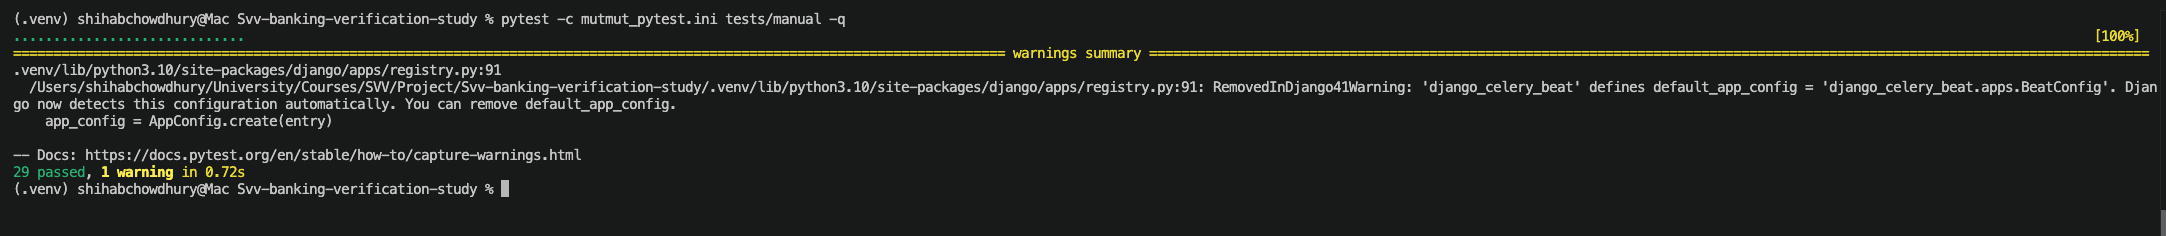
\includegraphics[width=0.96\textwidth]
    {figures/manual_pytest.png}
    \caption{Manual EP/BVA test-suite execution showing 29 passing tests.}
    \label{fig:manual-pytest-evidence}
\end{figure}

\subsection{Property-Based Test-Suite Evidence}

The Hypothesis property-based suite executed successfully with 16 passing test
functions.

\begin{figure}[H]
    \centering
    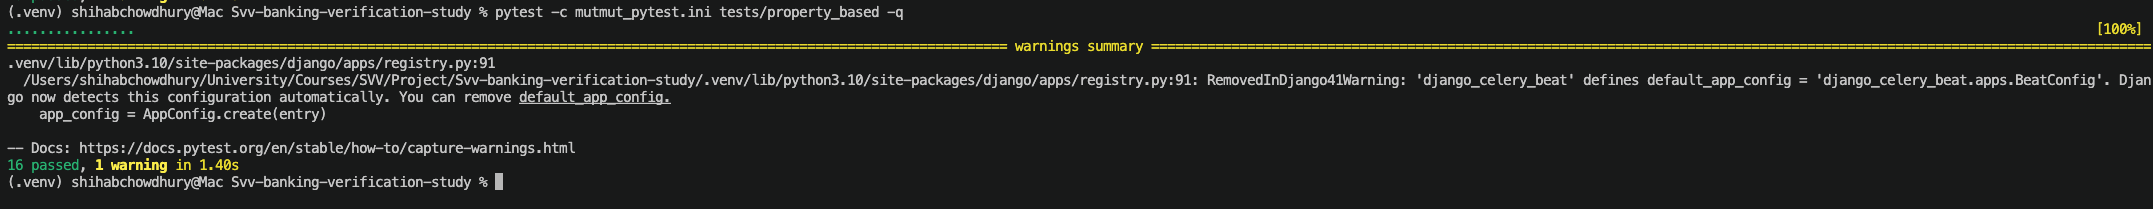
\includegraphics[width=0.96\textwidth]
    {figures/property_pytest.png}
    \caption{Property-based test-suite execution showing 16 passing tests.}
    \label{fig:property-pytest-evidence}
\end{figure}

\subsection{Coverage Evidence}

The manual suite achieved 84\% overall structural coverage.

\begin{figure}[H]
    \centering
    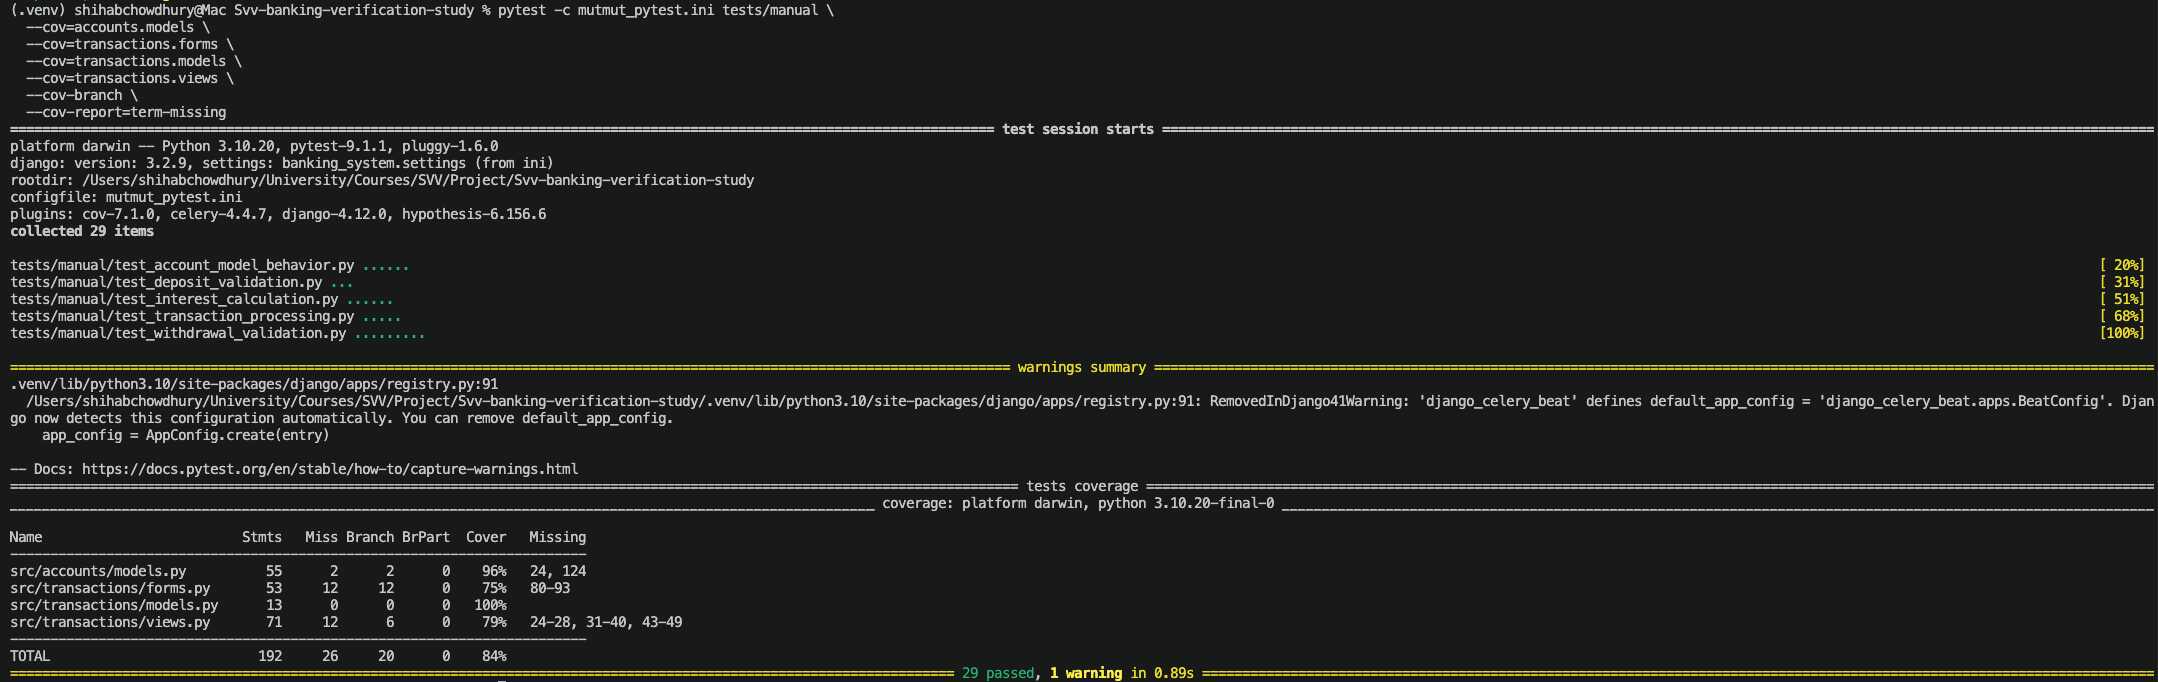
\includegraphics[width=0.96\textwidth]
    {figures/manual_coverage_output.png}
    \caption{Manual-suite statement and branch coverage output.}
    \label{fig:manual-coverage-evidence}
\end{figure}

The property-based suite achieved 77\% overall structural coverage.

\begin{figure}[H]
    \centering
    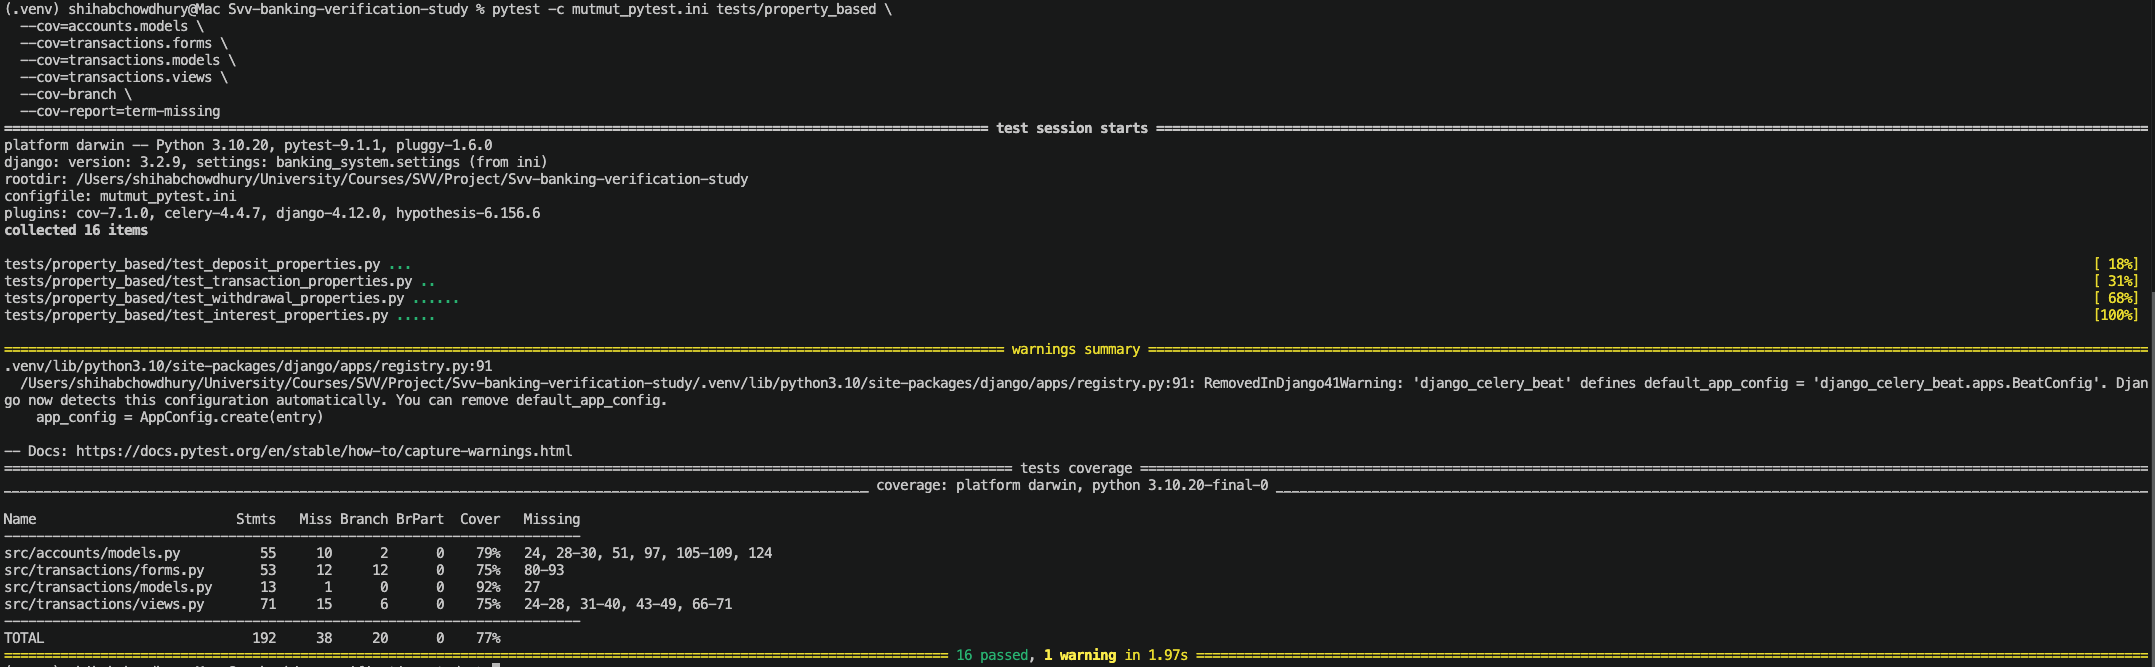
\includegraphics[width=0.96\textwidth]
    {figures/property_coverage_output.png}
    \caption{Property-based statement and branch coverage output.}
    \label{fig:property-coverage-evidence}
\end{figure}

\subsection{Mutation-Testing Evidence}

The manual mutation run produced 53 killed mutants, 17 surviving mutants,
26 no-test mutants, and no timeout mutants.

\begin{figure}[H]
    \centering
    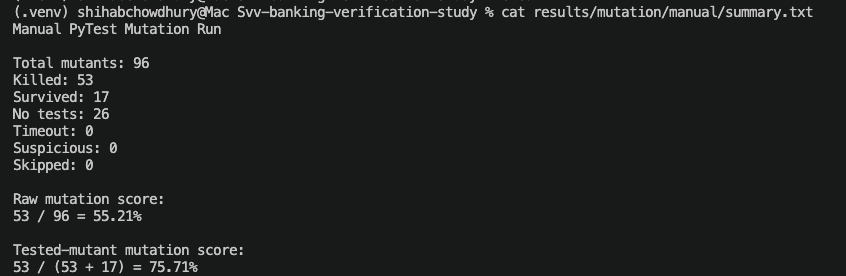
\includegraphics[width=0.96\textwidth]
    {figures/manual_mutation_output.png}
    \caption{Manual-suite mutation-testing summary.}
    \label{fig:manual-mutation-evidence}
\end{figure}

The property-based mutation run produced 42 killed mutants, 15 surviving
mutants, 39 no-test mutants, and no timeout mutants.

\begin{figure}[H]
    \centering
    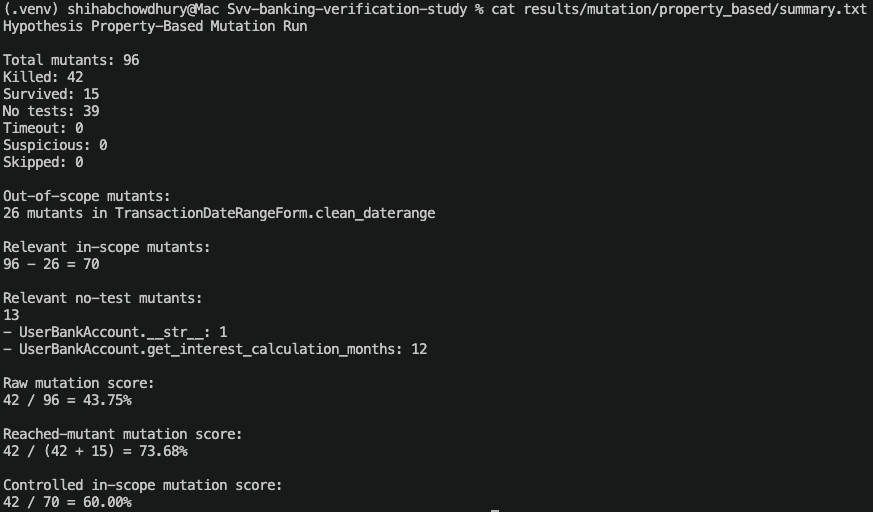
\includegraphics[width=0.96\textwidth]
    {figures/property_mutation_output.png}
    \caption{Property-based mutation-testing summary.}
    \label{fig:property-mutation-evidence}
\end{figure}

\bibliographystyle{IEEEtran}
\bibliography{references}
\end{document}